\documentclass[11pt]{article}
\newcommand{\tablelang}{uk}
% Ukrainian theorem names (picked up by \providecommand in preamble.tex)
\newcommand{\lemmaname}{Лема}
\newcommand{\propositionname}{Твердження}
\newcommand{\definitionname}{Означення}
\newcommand{\remarkname}{Зауваження}
\newcommand{\theoremname}{Теорема}
\newcommand{\corollaryname}{Наслідок}
% Shared preamble for paper/tex/en/main.tex and paper/tex/uk/main.tex (XeLaTeX via Tectonic).
% The including file sets \mainlang{english} or \mainlang{ukrainian} before % Shared preamble for paper/tex/en/main.tex and paper/tex/uk/main.tex (XeLaTeX via Tectonic).
% The including file sets \mainlang{english} or \mainlang{ukrainian} before % Shared preamble for paper/tex/en/main.tex and paper/tex/uk/main.tex (XeLaTeX via Tectonic).
% The including file sets \mainlang{english} or \mainlang{ukrainian} before \input{../preamble}.
\usepackage[a4paper,margin=25mm]{geometry}
\usepackage{fontspec}
\setmainfont{cmunrm.otf}[BoldFont=cmunbx.otf,ItalicFont=cmunti.otf,BoldItalicFont=cmunbi.otf]
\setsansfont{cmunss.otf}[BoldFont=cmunsx.otf,ItalicFont=cmunsi.otf]
\setmonofont{cmuntt.otf}[BoldFont=cmuntb.otf,ItalicFont=cmunit.otf]
\usepackage[ukrainian,english]{babel}
\usepackage{amsmath,amssymb,amsthm,mathtools}
\usepackage{booktabs,tabularx,array,multirow}
\usepackage{graphicx}
\usepackage[font=small,labelfont=bf]{caption}
\usepackage{subcaption}
\usepackage{xcolor}
\usepackage{microtype}
\usepackage[numbers,sort&compress]{natbib}
\PassOptionsToPackage{hyphens}{url}
\usepackage[hidelinks]{hyperref}
\usepackage[nameinlink,capitalise,noabbrev]{cleveref}
\usepackage{url}

\graphicspath{{../../figures/}}
% primitive input: LaTeX's \input is not expandable and breaks inside tabular after \midrule
\makeatletter\newcommand{\gentable}[1]{\@@input ../tables/\tablelang/T#1.tex }\makeatother

% notation
\newcommand{\Q}{\mathbb{Q}}
\newcommand{\Fp}{\mathbb{F}_p}
\newcommand{\C}{\mathbb{C}}
\newcommand{\Dh}{D_H}
\newcommand{\Dmid}{D_{\mathrm{mid}}}
\newcommand{\T}{\mathsf{T}}
\newcommand{\Cl}{\operatorname{Cl}_2}
\newcommand{\dft}{\operatorname{DFT}}
\newcommand{\code}[1]{\texttt{#1}}

% theorem names: the including file may define these before \input{../preamble}
\providecommand{\lemmaname}{Lemma}
\providecommand{\propositionname}{Proposition}
\providecommand{\definitionname}{Definition}
\providecommand{\remarkname}{Remark}
\providecommand{\corollaryname}{Corollary}
\providecommand{\theoremname}{Theorem}
\theoremstyle{plain}
\newtheorem{lemma}{\lemmaname}
\newtheorem{proposition}{\propositionname}
\theoremstyle{definition}
\newtheorem{definition}{\definitionname}
\theoremstyle{remark}
\newtheorem{remark}{\remarkname}

\setlength{\tabcolsep}{4pt}
\renewcommand{\arraystretch}{1.12}
\sloppy
.
\usepackage[a4paper,margin=25mm]{geometry}
\usepackage{fontspec}
\setmainfont{cmunrm.otf}[BoldFont=cmunbx.otf,ItalicFont=cmunti.otf,BoldItalicFont=cmunbi.otf]
\setsansfont{cmunss.otf}[BoldFont=cmunsx.otf,ItalicFont=cmunsi.otf]
\setmonofont{cmuntt.otf}[BoldFont=cmuntb.otf,ItalicFont=cmunit.otf]
\usepackage[ukrainian,english]{babel}
\usepackage{amsmath,amssymb,amsthm,mathtools}
\usepackage{booktabs,tabularx,array,multirow}
\usepackage{graphicx}
\usepackage[font=small,labelfont=bf]{caption}
\usepackage{subcaption}
\usepackage{xcolor}
\usepackage{microtype}
\usepackage[numbers,sort&compress]{natbib}
\PassOptionsToPackage{hyphens}{url}
\usepackage[hidelinks]{hyperref}
\usepackage[nameinlink,capitalise,noabbrev]{cleveref}
\usepackage{url}

\graphicspath{{../../figures/}}
% primitive input: LaTeX's \input is not expandable and breaks inside tabular after \midrule
\makeatletter\newcommand{\gentable}[1]{\@@input ../tables/\tablelang/T#1.tex }\makeatother

% notation
\newcommand{\Q}{\mathbb{Q}}
\newcommand{\Fp}{\mathbb{F}_p}
\newcommand{\C}{\mathbb{C}}
\newcommand{\Dh}{D_H}
\newcommand{\Dmid}{D_{\mathrm{mid}}}
\newcommand{\T}{\mathsf{T}}
\newcommand{\Cl}{\operatorname{Cl}_2}
\newcommand{\dft}{\operatorname{DFT}}
\newcommand{\code}[1]{\texttt{#1}}

% theorem names: the including file may define these before % Shared preamble for paper/tex/en/main.tex and paper/tex/uk/main.tex (XeLaTeX via Tectonic).
% The including file sets \mainlang{english} or \mainlang{ukrainian} before \input{../preamble}.
\usepackage[a4paper,margin=25mm]{geometry}
\usepackage{fontspec}
\setmainfont{cmunrm.otf}[BoldFont=cmunbx.otf,ItalicFont=cmunti.otf,BoldItalicFont=cmunbi.otf]
\setsansfont{cmunss.otf}[BoldFont=cmunsx.otf,ItalicFont=cmunsi.otf]
\setmonofont{cmuntt.otf}[BoldFont=cmuntb.otf,ItalicFont=cmunit.otf]
\usepackage[ukrainian,english]{babel}
\usepackage{amsmath,amssymb,amsthm,mathtools}
\usepackage{booktabs,tabularx,array,multirow}
\usepackage{graphicx}
\usepackage[font=small,labelfont=bf]{caption}
\usepackage{subcaption}
\usepackage{xcolor}
\usepackage{microtype}
\usepackage[numbers,sort&compress]{natbib}
\PassOptionsToPackage{hyphens}{url}
\usepackage[hidelinks]{hyperref}
\usepackage[nameinlink,capitalise,noabbrev]{cleveref}
\usepackage{url}

\graphicspath{{../../figures/}}
% primitive input: LaTeX's \input is not expandable and breaks inside tabular after \midrule
\makeatletter\newcommand{\gentable}[1]{\@@input ../tables/\tablelang/T#1.tex }\makeatother

% notation
\newcommand{\Q}{\mathbb{Q}}
\newcommand{\Fp}{\mathbb{F}_p}
\newcommand{\C}{\mathbb{C}}
\newcommand{\Dh}{D_H}
\newcommand{\Dmid}{D_{\mathrm{mid}}}
\newcommand{\T}{\mathsf{T}}
\newcommand{\Cl}{\operatorname{Cl}_2}
\newcommand{\dft}{\operatorname{DFT}}
\newcommand{\code}[1]{\texttt{#1}}

% theorem names: the including file may define these before \input{../preamble}
\providecommand{\lemmaname}{Lemma}
\providecommand{\propositionname}{Proposition}
\providecommand{\definitionname}{Definition}
\providecommand{\remarkname}{Remark}
\providecommand{\corollaryname}{Corollary}
\providecommand{\theoremname}{Theorem}
\theoremstyle{plain}
\newtheorem{lemma}{\lemmaname}
\newtheorem{proposition}{\propositionname}
\theoremstyle{definition}
\newtheorem{definition}{\definitionname}
\theoremstyle{remark}
\newtheorem{remark}{\remarkname}

\setlength{\tabcolsep}{4pt}
\renewcommand{\arraystretch}{1.12}
\sloppy

\providecommand{\lemmaname}{Lemma}
\providecommand{\propositionname}{Proposition}
\providecommand{\definitionname}{Definition}
\providecommand{\remarkname}{Remark}
\providecommand{\corollaryname}{Corollary}
\providecommand{\theoremname}{Theorem}
\theoremstyle{plain}
\newtheorem{lemma}{\lemmaname}
\newtheorem{proposition}{\propositionname}
\theoremstyle{definition}
\newtheorem{definition}{\definitionname}
\theoremstyle{remark}
\newtheorem{remark}{\remarkname}

\setlength{\tabcolsep}{4pt}
\renewcommand{\arraystretch}{1.12}
\sloppy
.
\usepackage[a4paper,margin=25mm]{geometry}
\usepackage{fontspec}
\setmainfont{cmunrm.otf}[BoldFont=cmunbx.otf,ItalicFont=cmunti.otf,BoldItalicFont=cmunbi.otf]
\setsansfont{cmunss.otf}[BoldFont=cmunsx.otf,ItalicFont=cmunsi.otf]
\setmonofont{cmuntt.otf}[BoldFont=cmuntb.otf,ItalicFont=cmunit.otf]
\usepackage[ukrainian,english]{babel}
\usepackage{amsmath,amssymb,amsthm,mathtools}
\usepackage{booktabs,tabularx,array,multirow}
\usepackage{graphicx}
\usepackage[font=small,labelfont=bf]{caption}
\usepackage{subcaption}
\usepackage{xcolor}
\usepackage{microtype}
\usepackage[numbers,sort&compress]{natbib}
\PassOptionsToPackage{hyphens}{url}
\usepackage[hidelinks]{hyperref}
\usepackage[nameinlink,capitalise,noabbrev]{cleveref}
\usepackage{url}

\graphicspath{{../../figures/}}
% primitive input: LaTeX's \input is not expandable and breaks inside tabular after \midrule
\makeatletter\newcommand{\gentable}[1]{\@@input ../tables/\tablelang/T#1.tex }\makeatother

% notation
\newcommand{\Q}{\mathbb{Q}}
\newcommand{\Fp}{\mathbb{F}_p}
\newcommand{\C}{\mathbb{C}}
\newcommand{\Dh}{D_H}
\newcommand{\Dmid}{D_{\mathrm{mid}}}
\newcommand{\T}{\mathsf{T}}
\newcommand{\Cl}{\operatorname{Cl}_2}
\newcommand{\dft}{\operatorname{DFT}}
\newcommand{\code}[1]{\texttt{#1}}

% theorem names: the including file may define these before % Shared preamble for paper/tex/en/main.tex and paper/tex/uk/main.tex (XeLaTeX via Tectonic).
% The including file sets \mainlang{english} or \mainlang{ukrainian} before % Shared preamble for paper/tex/en/main.tex and paper/tex/uk/main.tex (XeLaTeX via Tectonic).
% The including file sets \mainlang{english} or \mainlang{ukrainian} before \input{../preamble}.
\usepackage[a4paper,margin=25mm]{geometry}
\usepackage{fontspec}
\setmainfont{cmunrm.otf}[BoldFont=cmunbx.otf,ItalicFont=cmunti.otf,BoldItalicFont=cmunbi.otf]
\setsansfont{cmunss.otf}[BoldFont=cmunsx.otf,ItalicFont=cmunsi.otf]
\setmonofont{cmuntt.otf}[BoldFont=cmuntb.otf,ItalicFont=cmunit.otf]
\usepackage[ukrainian,english]{babel}
\usepackage{amsmath,amssymb,amsthm,mathtools}
\usepackage{booktabs,tabularx,array,multirow}
\usepackage{graphicx}
\usepackage[font=small,labelfont=bf]{caption}
\usepackage{subcaption}
\usepackage{xcolor}
\usepackage{microtype}
\usepackage[numbers,sort&compress]{natbib}
\PassOptionsToPackage{hyphens}{url}
\usepackage[hidelinks]{hyperref}
\usepackage[nameinlink,capitalise,noabbrev]{cleveref}
\usepackage{url}

\graphicspath{{../../figures/}}
% primitive input: LaTeX's \input is not expandable and breaks inside tabular after \midrule
\makeatletter\newcommand{\gentable}[1]{\@@input ../tables/\tablelang/T#1.tex }\makeatother

% notation
\newcommand{\Q}{\mathbb{Q}}
\newcommand{\Fp}{\mathbb{F}_p}
\newcommand{\C}{\mathbb{C}}
\newcommand{\Dh}{D_H}
\newcommand{\Dmid}{D_{\mathrm{mid}}}
\newcommand{\T}{\mathsf{T}}
\newcommand{\Cl}{\operatorname{Cl}_2}
\newcommand{\dft}{\operatorname{DFT}}
\newcommand{\code}[1]{\texttt{#1}}

% theorem names: the including file may define these before \input{../preamble}
\providecommand{\lemmaname}{Lemma}
\providecommand{\propositionname}{Proposition}
\providecommand{\definitionname}{Definition}
\providecommand{\remarkname}{Remark}
\providecommand{\corollaryname}{Corollary}
\providecommand{\theoremname}{Theorem}
\theoremstyle{plain}
\newtheorem{lemma}{\lemmaname}
\newtheorem{proposition}{\propositionname}
\theoremstyle{definition}
\newtheorem{definition}{\definitionname}
\theoremstyle{remark}
\newtheorem{remark}{\remarkname}

\setlength{\tabcolsep}{4pt}
\renewcommand{\arraystretch}{1.12}
\sloppy
.
\usepackage[a4paper,margin=25mm]{geometry}
\usepackage{fontspec}
\setmainfont{cmunrm.otf}[BoldFont=cmunbx.otf,ItalicFont=cmunti.otf,BoldItalicFont=cmunbi.otf]
\setsansfont{cmunss.otf}[BoldFont=cmunsx.otf,ItalicFont=cmunsi.otf]
\setmonofont{cmuntt.otf}[BoldFont=cmuntb.otf,ItalicFont=cmunit.otf]
\usepackage[ukrainian,english]{babel}
\usepackage{amsmath,amssymb,amsthm,mathtools}
\usepackage{booktabs,tabularx,array,multirow}
\usepackage{graphicx}
\usepackage[font=small,labelfont=bf]{caption}
\usepackage{subcaption}
\usepackage{xcolor}
\usepackage{microtype}
\usepackage[numbers,sort&compress]{natbib}
\PassOptionsToPackage{hyphens}{url}
\usepackage[hidelinks]{hyperref}
\usepackage[nameinlink,capitalise,noabbrev]{cleveref}
\usepackage{url}

\graphicspath{{../../figures/}}
% primitive input: LaTeX's \input is not expandable and breaks inside tabular after \midrule
\makeatletter\newcommand{\gentable}[1]{\@@input ../tables/\tablelang/T#1.tex }\makeatother

% notation
\newcommand{\Q}{\mathbb{Q}}
\newcommand{\Fp}{\mathbb{F}_p}
\newcommand{\C}{\mathbb{C}}
\newcommand{\Dh}{D_H}
\newcommand{\Dmid}{D_{\mathrm{mid}}}
\newcommand{\T}{\mathsf{T}}
\newcommand{\Cl}{\operatorname{Cl}_2}
\newcommand{\dft}{\operatorname{DFT}}
\newcommand{\code}[1]{\texttt{#1}}

% theorem names: the including file may define these before % Shared preamble for paper/tex/en/main.tex and paper/tex/uk/main.tex (XeLaTeX via Tectonic).
% The including file sets \mainlang{english} or \mainlang{ukrainian} before \input{../preamble}.
\usepackage[a4paper,margin=25mm]{geometry}
\usepackage{fontspec}
\setmainfont{cmunrm.otf}[BoldFont=cmunbx.otf,ItalicFont=cmunti.otf,BoldItalicFont=cmunbi.otf]
\setsansfont{cmunss.otf}[BoldFont=cmunsx.otf,ItalicFont=cmunsi.otf]
\setmonofont{cmuntt.otf}[BoldFont=cmuntb.otf,ItalicFont=cmunit.otf]
\usepackage[ukrainian,english]{babel}
\usepackage{amsmath,amssymb,amsthm,mathtools}
\usepackage{booktabs,tabularx,array,multirow}
\usepackage{graphicx}
\usepackage[font=small,labelfont=bf]{caption}
\usepackage{subcaption}
\usepackage{xcolor}
\usepackage{microtype}
\usepackage[numbers,sort&compress]{natbib}
\PassOptionsToPackage{hyphens}{url}
\usepackage[hidelinks]{hyperref}
\usepackage[nameinlink,capitalise,noabbrev]{cleveref}
\usepackage{url}

\graphicspath{{../../figures/}}
% primitive input: LaTeX's \input is not expandable and breaks inside tabular after \midrule
\makeatletter\newcommand{\gentable}[1]{\@@input ../tables/\tablelang/T#1.tex }\makeatother

% notation
\newcommand{\Q}{\mathbb{Q}}
\newcommand{\Fp}{\mathbb{F}_p}
\newcommand{\C}{\mathbb{C}}
\newcommand{\Dh}{D_H}
\newcommand{\Dmid}{D_{\mathrm{mid}}}
\newcommand{\T}{\mathsf{T}}
\newcommand{\Cl}{\operatorname{Cl}_2}
\newcommand{\dft}{\operatorname{DFT}}
\newcommand{\code}[1]{\texttt{#1}}

% theorem names: the including file may define these before \input{../preamble}
\providecommand{\lemmaname}{Lemma}
\providecommand{\propositionname}{Proposition}
\providecommand{\definitionname}{Definition}
\providecommand{\remarkname}{Remark}
\providecommand{\corollaryname}{Corollary}
\providecommand{\theoremname}{Theorem}
\theoremstyle{plain}
\newtheorem{lemma}{\lemmaname}
\newtheorem{proposition}{\propositionname}
\theoremstyle{definition}
\newtheorem{definition}{\definitionname}
\theoremstyle{remark}
\newtheorem{remark}{\remarkname}

\setlength{\tabcolsep}{4pt}
\renewcommand{\arraystretch}{1.12}
\sloppy

\providecommand{\lemmaname}{Lemma}
\providecommand{\propositionname}{Proposition}
\providecommand{\definitionname}{Definition}
\providecommand{\remarkname}{Remark}
\providecommand{\corollaryname}{Corollary}
\providecommand{\theoremname}{Theorem}
\theoremstyle{plain}
\newtheorem{lemma}{\lemmaname}
\newtheorem{proposition}{\propositionname}
\theoremstyle{definition}
\newtheorem{definition}{\definitionname}
\theoremstyle{remark}
\newtheorem{remark}{\remarkname}

\setlength{\tabcolsep}{4pt}
\renewcommand{\arraystretch}{1.12}
\sloppy

\providecommand{\lemmaname}{Lemma}
\providecommand{\propositionname}{Proposition}
\providecommand{\definitionname}{Definition}
\providecommand{\remarkname}{Remark}
\providecommand{\corollaryname}{Corollary}
\providecommand{\theoremname}{Theorem}
\theoremstyle{plain}
\newtheorem{lemma}{\lemmaname}
\newtheorem{proposition}{\propositionname}
\theoremstyle{definition}
\newtheorem{definition}{\definitionname}
\theoremstyle{remark}
\newtheorem{remark}{\remarkname}

\setlength{\tabcolsep}{4pt}
\renewcommand{\arraystretch}{1.12}
\sloppy


% ---- additions local to the Ukrainian article (preamble.tex left unchanged) ----
\theoremstyle{plain}
\newtheorem{theorem}{Теорема}
\newtheorem{corollary}{Наслідок}
\DeclareMathOperator{\diag}{diag}
\DeclareMathOperator{\lcm}{lcm}
\newcommand{\abs}[1]{\lvert #1\rvert}
\newcommand{\norm}[1]{\lVert #1\rVert}
\newcommand{\Z}{\mathbb{Z}}
\newcommand{\hd}[1]{\begin{tabular}[b]{@{}c@{}}#1\end{tabular}}
\newcommand{\hdl}[1]{\begin{tabular}[b]{@{}l@{}}#1\end{tabular}}
\newcolumntype{L}{>{\raggedright\arraybackslash}X}
\newcolumntype{P}[1]{>{\raggedright\arraybackslash}p{#1}}
\newcommand{\en}[1]{\foreignlanguage{english}{#1}}
% Ukrainian cleveref names (cleveref has no Ukrainian support)
\crefname{section}{розділ}{розділи}
\Crefname{section}{Розділ}{Розділи}
\crefname{subsection}{підрозділ}{підрозділи}
\Crefname{subsection}{Підрозділ}{Підрозділи}
\crefname{subsubsection}{підрозділ}{підрозділи}
\Crefname{subsubsection}{Підрозділ}{Підрозділи}
\crefname{appendix}{додаток}{додатки}
\Crefname{appendix}{Додаток}{Додатки}
\crefname{subappendix}{додаток}{додатки}
\Crefname{subappendix}{Додаток}{Додатки}
\crefname{table}{таблиця}{таблиці}
\Crefname{table}{Таблиця}{Таблиці}
\crefname{figure}{рисунок}{рисунки}
\Crefname{figure}{Рисунок}{Рисунки}
\crefname{equation}{формула}{формули}
\Crefname{equation}{Формула}{Формули}
\crefname{lemma}{лема}{леми}
\Crefname{lemma}{Лема}{Леми}
\crefname{proposition}{твердження}{твердження}
\Crefname{proposition}{Твердження}{Твердження}
\crefname{theorem}{теорема}{теореми}
\Crefname{theorem}{Теорема}{Теореми}
\crefname{corollary}{наслідок}{наслідки}
\Crefname{corollary}{Наслідок}{Наслідки}
\crefname{definition}{означення}{означення}
\Crefname{definition}{Означення}{Означення}
\crefname{remark}{зауваження}{зауваження}
\Crefname{remark}{Зауваження}{Зауваження}
\setlength{\emergencystretch}{2em}
\hypersetup{pdftitle={Незалежна перевірка локального компілятора Фур'є з препринту OpenAI},pdfauthor={Олександр Пилипенко}}

\begin{document}
\selectlanguage{ukrainian}
\renewcommand{\crefpairconjunction}{ і }
\renewcommand{\crefmiddleconjunction}{, }
\renewcommand{\creflastconjunction}{ і }
\renewcommand{\crefpairgroupconjunction}{ і }
\renewcommand{\crefmiddlegroupconjunction}{, }
\renewcommand{\creflastgroupconjunction}{ і }
\renewcommand{\crefrangeconjunction}{--}

\title{Незалежна перевірка локального компілятора Фур'є з препринту OpenAI
«\en{An explicit power saving for the exact discrete Fourier transform}»:
точні й чисельні тести, глибина, вартість і межі застосовності}
\author{Олександр Пилипенко\\[2pt]\small ORCID: \href{https://orcid.org/0009-0004-9610-9242}{0009-0004-9610-9242}\\ \href{mailto:op1@cyberunit.tech}{\texttt{op1@cyberunit.tech}}, \href{mailto:limblucifer666@gmail.com}{\texttt{limblucifer666@gmail.com}}}
\date{2026-10-14}
\maketitle

\begin{abstract}
\noindent
Ми незалежно перевіряємо одну складову препринту OpenAI «\en{An explicit power saving for the exact discrete Fourier transform}», який стверджує існування точного детермінованого алгоритму DFT для кожної довжини $n$ за час $O\bigl(n(\log n)^{\theta}(\log\log n)^{4-\theta}\bigr)$, $\theta=1-2{,}1\cdot10^{-13}$, з точною комплексною арифметикою і необмеженими коефіцієнтами. Показник дає тензорна мережа, яку ми не реалізовували. Ми реалізували локальний компілятор Фур'є (ньютонову редукцію $F_r(u)$ до трикутних Тепліцевих множників, блочне Тепліцеве слово точної ширини з реплеєм згорткових DAG і шаблон зсувів з $C$-слотами), чия межа $O(\log^4 r)$ слотів дає множник $(\log\log n)^4$, а не $\theta$. Усі результати стосуються строгої конструкції, топологія якої залежить лише від ширини. Обчислення в $\Q(\zeta_N)$ доводить, що реалізована матриця дорівнює $F_r(u)$ при $r=4,7,8,9,12,15,16,32$ (шлях через $C$-слоти~--- при $r=4,8,16$). Точні образи в $\Fp$ збігаються на вибраних ширинах до 512, а в потоковому тесті~--- і при $r=1024$; це лише необхідна умова. Дві точності mpmath, що відрізняються на 100 знаків, зменшують похибку приблизно на 100 порядків на всіх ширинах 7--256. Хоча $\kappa_2(F_r)=1$, слово числово нестійке: $\log_{10}\kappa_2(\Dh)$ має головний член $cr$, $c=\Cl(\pi/3)/(\pi\ln10)\approx0{,}1403$, ланцюжок втрачає 142 знаки при $r=256$, а у float64 відносна похибка при $r=64$ сягає $8\cdot10^{23}$; препринт не робить тверджень про скінченну точність. Хеші структури збігаються для трьох входів на 12 ширинах 64--1024, а модель глибини точно збігається з виміряною ASAP-глибиною на 10 із них. Ми також перекомпілювали Lean-формалізацію OpenAI і провели аудит її формулювання.
\end{abstract}

\noindent\textbf{Ключові слова:} дискретне перетворення Фур'є; схемна складність; глибина схеми; Тепліцева матриця; числова стійкість; циклотомічні поля; точна арифметика; формальна верифікація (Lean).

\medskip
\noindent\textbf{Заява про незалежність.} Це незалежна перевірка частини препринту OpenAI. Станом на 2026-10-14 контакту з OpenAI щодо цієї роботи не було; перевірку не узгоджували з авторами препринту, і вони її не рецензували. Нового алгоритму DFT не запропоновано.

% =====================================================================
\section{Вступ}\label{sec:intro}

\subsection{Мотивація}
Препринт OpenAI~\citep{openai2026} стверджує, що DFT довжини $n$ можна обчислити точно за час $o(n\log n)$ у моделі з одиничною вартістю арифметичних операцій над комплексними числами і одиничною вартістю цілочисельних операцій над словами з $O(\log n)$ біт. Алгоритм Кулі--Тьюкі~\citep{cooley1965} дає $O(n\log n)$. Відомі нижні межі для суміжних моделей~\citep{morgenstern1973,ailon2013,ailon2014} не переносяться на цю модель автоматично (підрозділ~\ref{sec:lower-bounds}). Твердження незвичне. Сам препринт застерігає, що сталі алгоритму величезні, що результат асимптотичний, «\en{with no useful crossover estimate}», і що висновок не стосується стійких FFT з плаваючою комою чи бітової складності (\code{introduction.tex:101}). Схожі практичні зауваження робить Recht~\citep{recht2026} (приховані сталі; точна арифметика над числами, що ростуть). Тому варто незалежно перевірити хоча б ті частини доведення, які можна перевірити обчисленням, і виміряти, як у них проявляються обмеження моделі, що їх препринт називає сам.

\paragraph{Джерело та авторство.}
Препринт не є окремою статтею з DOI. Це текст у репозиторії \url{https://github.com/openai/math}, каталог \path{preprints/An-explicit-power-saving-for-the-exact-discrete-Fourier-transform-September-25-2026}: головний файл \code{main.pdf}, вихідні файли \code{build/main.tex}, розділи \code{build/sections/*.tex} і бібліографія \code{build/references.bib}. Ми працювали зі станом каталогу на коміті 301488868 (2026-10-07; HEAD репозиторію fd4aeeb) і посилаємося на твердження за їхніми мітками (\code{thm:main}, \code{cor:decimal}, \code{loc:compiler}, \dots), а на рядки джерел~--- у вигляді \code{file.tex:line}. В авторському блоці і в README каталогу автором зазначено «OpenAI» (\code{build/main.tex}, \verb|\author{OpenAI}|; \code{README.md}, «Author: OpenAI»); іменних авторів немає. За README репозиторію, рукописи колекції створено внутрішньою моделлю OpenAI. Lean-формалізація, яку ми перекомпілювали (підрозділ~\ref{sec:lean}),~--- окремий артефакт того самого репозиторію (каталог \code{lean/}, опис обсягу~--- \code{lean/docs/130.md}), а не частина тексту препринту.

\subsection{Що перевіряється}
Ми перевіряємо локальний компілятор з \code{local.tex}: правильність реалізованого оператора (точно і в арифметиці високої точності), його числову поведінку, глибину за ASAP-розкладом і вартість. Наші локальні експерименти не відтворюють головної теореми й не перевіряють асимптотичного виграшу з показником $\theta$; окремо ми відтворили механічну перевірку Lean-цілі (підрозділ~\ref{sec:lean}). У таблиці~\ref{tab:status} підсумовано статус кожної складової препринту.

Сила доказу різна, і ми розрізняємо її рівні (підрозділ~\ref{sec:evidence}). За спаданням: (1)~\emph{доведення обчисленням}, тобто точна рівність у $\Q(\zeta_N)$ для восьми ширин 4--32 (повний ланцюжок) і для $r=4,8,16$ ($C$-слоти); (2)~\emph{точні, але лише необхідні умови}, тобто рівність образів у $\Fp$ для вибраних ширин до 512; (3)~\emph{числова узгодженість}, тобто mpmath з двома точностями до $r=256$; (4)~\emph{вимірювання конкретного слова}: топологія, ASAP-глибина, гейти, флопи, час. Локальними експериментами не перевірено: мережу, асимптотичний виграш із $\theta$, синхронізацію, довжини всіх розмірів, синтез. Наші результати не підтверджують і не спростовують головної теореми.

\begin{table}[tb]
\centering\small
\caption{Статус складових препринту в цьому дослідженні.}\label{tab:status}
\begin{tabularx}{\linewidth}{@{}P{0.25\linewidth}LL@{}}
\toprule
Складова (файл / мітка препринту) & Що зроблено тут & Статус \\
\midrule
Ньютонова редукція (\code{loc:newton-reduction}) & Повний ланцюжок DFT: точно в $\Q(\zeta_N)$ і $\Fp$; у mp з двома точностями & Доведення обчисленням для всієї матриці при $r=4,7,8,9,12,15,16,32$ ($\Q(\zeta_N)$); необхідна умова на вибраних $r\le128$ ($\Fp$) \\
Тепліцеве слово (\code{loc:toeplitz}), строгий режим & Глибина, гейти, топологія (аудит), точність $Tx$ & Виміряно на вибраних ширинах до $r=1024$; точність і обсяг~--- \cref{tab:exact,tab:mp,tab:cslots,tab:float,tab:cond,tab:stage,tab:randtoep,tab:roots,tab:depth,tab:model} \\
Реплей DAG (\code{loc:replay}) & Виконання за раундами дорівнює послідовному; конфліктів немає & Перевірено (строгий режим) \\
Шаблон $C$-слотів (\code{loc:compiler}) & Власний замкнений розклад зсуву; розщеплення без тесту на нуль; спряження через DAG з оберненими коренями & Доведення обчисленням при $r=4,8,16$ ($\Q(\zeta_N)$); необхідна умова на вибраних $r\le128$ ($\Fp$); mp до $r=256$ \\
Правило розміру чанка & Еквівалентне правилу препринту для $b\le1024$ (підрозділ~\ref{sec:chunk}) & Перевірено для $b\le1024$ \\
Конкретна мережа з \code{network.tex} та її асимптотичний виграш & Не реалізовано; числове $\theta$ перераховано (підрозділ~\ref{sec:constants}); Lean для іншої мережі~--- у підрозділі~\ref{sec:lean} & Локальними експериментами не перевірено \\
Синхронізація (\code{synchronization.tex}) & Не реалізовано & Не перевірено \\
Довжини всіх розмірів (\code{all-lengths.tex}) & Не реалізовано & Не перевірено \\
Синтез і принтер (\code{synthesis.tex}) & Не реалізовано & Не перевірено \\
Lean-формалізація (\path{lean/OAI/Computability/FourierTransform}) & Скомпільовано: 0 помилок, 0 попереджень про \code{sorry}; аксіоми лише \code{propext}, \code{Classical.choice}, \code{Quot.sound} & Механічно перевірено; звірку означень завершено в заявленому обсязі; адекватність \code{Bill} і конкретна \code{network.tex}~--- поза аудитом \\
\bottomrule
\end{tabularx}
\end{table}

\subsection{Що не входить у роботу}
Ми не реалізовували і не перевіряли:
\begin{itemize}
\item мережу з \code{network.tex} (бінарні рамки, бюджет вимірів, тензорний степінь ядра $C$ і лему \code{net:tensor-bound}, з якої походить $\theta$);
\item синхронізацію тензорних множників (\code{synchronization.tex});
\item довжини всіх розмірів через китайську теорему про залишки і чирп-згортку (\code{all-lengths.tex});
\item синтез і принтер (\code{synthesis.tex}).
\end{itemize}
Показник $\theta$ дає мережа, а не локальний компілятор. Локальний компілятор~--- необхідна складова доведення (його $O(\log^4 r)$ слотів дають множник $(\log\log n)^4$ головної межі; \code{synchronization.tex:74}, \code{all-lengths.tex:137}), але не джерело економії. Наші результати стосуються цієї складової, і переносити їх на головну теорему не можна.

\subsection{Внесок}
Ми не пропонуємо нового алгоритму DFT. Наш внесок~--- незалежна реалізація і перевірка локального компілятора Фур'є на вибраних ширинах, кількісне дослідження його числової нестійкості та відтворювані інструменти точної перевірки, зокрема потокове обчислення великих обчислювальних графів. Конкретно, дослідження дає:
\begin{enumerate}
\item[(а)] Відтворювану реалізацію і перевірку повного ланцюжка ньютонової редукції і Тепліцевого слова для DFT: точно в циклотомічних і скінченних полях та в арифметиці високої точності, з окремими тестами загального Тепліцевого оператора і шляху через $C$-слоти. Рівні доказовості і перевірені ширини наведено в підрозділі~\ref{sec:evidence}.
\item[(б)] Незалежно виведений алгебраїчний розклад зсуву через $C$-слоти; матричну тотожність і умови ненульовості параметрів доведено в підрозділі~\ref{sec:cslots}.
\item[(в)] Аналітичний опис обумовленості $\Dh$ у випадку Фур'є: точні скінченні часткові суми і головний асимптотичний член $cr$ для $\log_{10}\kappa_2(\Dh)$ через функцію Клаузена (додаток~\ref{app:clausen}).
\item[(г)] Кількісне дослідження втрати знаків по етапах, росту проміжних величин по рівнях рекурсії і фазах та чутливості похибки до точності фаз для перевірених входів (підрозділ~\ref{sec:stagewise}). Ці діагностики не дають повного причинного розкладу похибки округлення.
\item[(д)] Вимірювання глибини, роботи, часу і пам'яті строгої конструкції з перевіреною фіксованою топологією; порівняння з FFT і прямим множенням в однакових одиницях вартості; виявлення артефактів глибини, спричинених залежним від значень пропуском нульових множників у нашій реалізації (підрозділ~\ref{sec:strict}).
\item[(е)] Відтворюваний потоковий точний перевірник у скінченних полях, що обчислює пряме і транспоноване слова без матеріалізації всього графа, зокрема окрему перевірку при $r=1024$ на тих самих двох векторах у двох полях. Її обсяг залишається точним тестом необхідної умови, а не доведенням для всієї комплексної матриці.
\end{enumerate}
Цей внесок стосується незалежно розробленої реалізації, аналізу та інструментів перевірки; пріоритету щодо математичних тотожностей чи асимптотик обумовленості ми не заявляємо. Виміряні обмеження (\cref{sec:res-instability,sec:res-cost}) стосуються скінченної точності або окремого виконання локального слова~--- режимів, про які препринт тверджень не робить. Препринту вони не спростовують.

% =====================================================================
\section{Твердження препринту}\label{sec:claims}
Цей розділ іде за текстом препринту, а не за нашим його прочитанням.

\subsection{Модель обчислень}\label{sec:model}
За розділом «\en{Arithmetic model and main result}» препринту~\citep{openai2026}: є комплексні регістри і цілочисельні адресні регістри. Одна операція поля коштує одиницю. Цілочисельні операції та довільний доступ до пам'яті на словах з $O(\log(n+2))$ біт коштують одиницю. Дозволені додавання, віднімання і множення на підготовлені скаляри, які не залежать від вхідних даних. Ділення дозволене лише при підготовці скалярів, і знаменник має бути доведено ненульовим. Один явно заданий корінь з одиниці $\zeta_D$, $D=D_*<1024\,n^3$, подається з одиничною вартістю. Обмежень на модуль коефіцієнтів немає, а стійкості обчислень з плаваючою комою препринт не розглядає і не заявляє: «\en{There is no bound on complex coefficients or intermediate magnitudes, and no finite-precision or numerical-stability assertion}» (\code{introduction.tex:67}). Там само препринт застерігає, що сталі величезні, що корисної оцінки точки перетину немає і що висновок «\en{does not assert a corresponding improvement for stable floating-point FFTs or for bit complexity}» (\code{introduction.tex:101}).

\subsection{Сталі і показник}\label{sec:constants}
Препринт означує
\begin{equation}\label{eq:constants}
m=10^6,\qquad W_*=2^{71},\qquad \Delta=6871402692000000,\qquad \lambda=m-\frac{\Delta}{W_*},\qquad \theta=\log_m\lambda,
\end{equation}
тож $\theta=0{,}99999999999978935615699598\ldots<1$. Позначимо
\begin{equation}\label{eq:delta}
\delta=1-\theta\approx2{,}106\cdot10^{-13}.
\end{equation}
Ми незалежно перерахували $\theta$ (mpmath, 50 знаків) і отримали те саме значення.

\subsection{Головна теорема і десятковий наслідок}
\begin{theorem}[{\citep[Theorem~\code{thm:main}]{openai2026}}]\label{thm:main}
Існує один детермінований точний алгоритм, який для кожного $n$ і кожного $x\in\C^n$ обчислює $F_nx$ за час
\begin{equation}\label{eq:main-bound}
O\bigl(n(\log n)^{\theta}(\log\log n)^{4-\theta}\bigr)\qquad(n\to\infty).
\end{equation}
Час включає підготовку скалярів, побудову розкладу і роботу з індексами.
\end{theorem}

\begin{corollary}[{\citep[Corollary~\code{cor:decimal}]{openai2026}}]\label{cor:decimal}
У тій самій моделі перетворення обчислюється за час $O\bigl(n(\log n)^{1-10^{-13}}\bigr)$, тобто $o(n\log n)$.
\end{corollary}

\subsection{Місце локального компілятора}\label{sec:role}
Головну теорему отримано з мережі: \code{net:tensor-bound} застосовує $C^{\otimes k}$ до масиву довжини $2^k$ за час $O\bigl(2^k(k+1)^{\theta}\bigr)$. Локальний компілятор (\code{loc:compiler}) і Тепліцеве слово (\code{loc:toeplitz}) не дають $\theta$, але є необхідною частиною конструкції: слова для всіх осей доповнюються до $O\bigl((1+\log r_{\max})^4\bigr)$ слотів, кожен слот виконує мережа, і звідси множник $(\log\ell)^4$ у
\begin{equation}\label{eq:Tn}
T(n)=O\bigl(n\,\ell^{\theta}(\log\ell)^4\bigr),\qquad \ell=\Theta\Bigl(\frac{\log n}{\log\log n}\Bigr)
\end{equation}
(\code{synchronization.tex:74--82}; \code{all-lengths.tex:137}). Вартість самого локального слова в гейтах у межу не входить; входять лише кількість слотів і поліноміальна підготовка. Локальні ширини~--- перші $\ell$ непарних простих і один степінь двійки (\code{all-lengths.tex:13--56}). Препринт зазначає, що механізм Фур'є точної ширини спільний із розділом~3 супровідного препринту \emph{\en{Finite tensor savings and exact Fourier circuits}}~\citep{openai2026companion} (\code{introduction.tex:158}, \code{local.tex:10--11}).

\paragraph{Що стверджує \code{local.tex}.}
Для первісного кореня $r$-го степеня з одиниці $u$ покладемо $F_r(u)=(u^{ij})_{0\le i,j<r}$.
\begin{itemize}
\item \emph{Лема \code{loc:newton-reduction}.} $F_r(u)=N D_N^{-1}N^{\T}$, $D_N=\diag(N_{00},\dots,N_{r-1,r-1})$, де $N$~--- оборотна нижня трикутна матриця, що є добутком двох діагональних матриць і однієї нижньої трикутної Тепліцевої. За формулою \code{loc:newton}
\begin{equation}\label{eq:newton}
N_{ik}=(-1)^k u^{k(k-1)/2}\,\frac{H_i}{H_{i-k}},\qquad H_j=\prod_{s=1}^{j}(1-u^s),\quad H_0=1,
\end{equation}
тобто $N=\Dh\,T\,D_c$ з $D_c=\diag(c_k)$, $c_k=(-1)^k u^{k(k-1)/2}$, і $D_N=\diag(c_kH_k)$.
\item \emph{Лема \code{loc:toeplitz}.} Оборотна нижня трикутна Тепліцева матриця ширини $r$ має слово на рівно $r$ координатах з $O(1+\log^4 r)$ змішаними раундами; «\en{the topology depends only on $r$}». Це верхня межа; оцінки $\Theta(\log^4 r)$ препринт тут не стверджує.
\item \emph{Правило розміру чанка} (там само). Для кожного $b\in\{1,\dots,v\}$ інтервали розбиваються на чанки розміру $b$ (крім, можливо, останнього); для кожної пари друкується скелет DAG і рахуються його гейти $g$; $b$ допустиме, якщо $g+a+e\le v$ для кожної пари, де $a,e$~--- розміри цільового і джерельного чанків; обирається найбільше допустиме $b$. Якщо допустимого немає, використовується пряме слово.
\item \emph{Рекурентність глибини} в доведенні:
\begin{equation}\label{eq:depth-rec}
d(v)\le\max\bigl\{d(\lfloor v/2\rfloor),\,d(\lceil v/2\rceil)\bigr\}+O(1+\log^3 v).
\end{equation}
\item \emph{Шаблон слотів} (\code{loc:compiler}). Кожен верхній зсув з ненульовим коефіцієнтом $t$ має слово з трьома прямими копіями $C$ і діагональними множниками (формули \code{loc:three-kernel} і \code{loc:nonzero-shear}): з $H'=\bigl(\begin{smallmatrix}1&1\\1&-1\end{smallmatrix}\bigr)$
\begin{equation}\label{eq:K}
\begin{gathered}
K=H'\diag(2,1)H'\diag(-3,1)H'=\begin{pmatrix}-8&-10\\0&-6\end{pmatrix},\\
\begin{pmatrix}1&t\\0&1\end{pmatrix}=D_t\diag(-1/8,-1/6)\,K\,D_t^{-1},\qquad D_t=\diag(4t/5,1).
\end{gathered}
\end{equation}
Довільний коефіцієнт $\mu$ розщеплюється як
\begin{equation}\label{eq:split}
\kappa=1+\mu\bar\mu,\qquad t_1=\kappa,\qquad t_2=\mu-\kappa,
\end{equation}
обидва ненульові, що дає однаковий шаблон із шести $C$-слотів для кожного коефіцієнта. Спряжене $\bar\mu$ є підготовленим скаляром: той самий арифметичний DAG обчислюється вдруге з оберненими коренями.
\end{itemize}

\subsection{Нижні межі, згадані в препринті}\label{sec:lower-bounds}
Morgenstern~\citep{morgenstern1973} дає нижню межу для ненормованого перетворення з обмеженими коефіцієнтами. Ailon~\citep{ailon2013,ailon2014} дає межі для нормованого перетворення з унітарними гейтами $2\times2$ і для моделі з обмеженою обумовленістю. Модель препринту допускає необмежені коефіцієнти, тож ці межі не переносяться на неї автоматично. Це пояснює відсутність прямої суперечності, але саме по собі не підтверджує доведення.

\subsection{Пов'язані роботи}\label{sec:related}
Recht~\citep{recht2026} (2026-10-12) називає результат «галактичним»: приховані сталі роблять його нерелевантним на фізично досяжних розмірах, а модель вимагає множити довільно великі комплексні числа за одну операцію. Обидва обмеження препринт називає сам (\code{introduction.tex:67}, \code{:101}), тож ця критика стосується практичної цінності, а не правильності. Наші дані (\cref{sec:res-instability,sec:res-cost,sec:disc-theta}) кількісно описують саме ці обмеження для локальної складової, але не стосуються мережі і не встановлюють нижніх меж вартості будь-якої майбутньої модифікації. Displacement-конструкцію чанків препринт бере з роботи Kailath, Kung і Morf~\citep{kailath1979}. Нестійкість швидких методів для Тепліцевих систем відома давно (Bunch~\citep{bunch1985}); наш випадок інший (множення, а не розв'язання), але механізм схожий: великі проміжні величини. Обумовленість ньютонової форми залежить від порядку вузлів: природний порядок $u^0,u^1,\dots$ вузлів на колі дає експоненційний ріст, а порядок Леджа його пригнічує (Reichel~\citep{reichel1990}). Наша формула для $\kappa(\Dh)$ (підрозділ~\ref{sec:res-instability}) кількісно описує саме природний порядок, який використовує препринт. Чи можна змінити порядок вузлів, не порушивши симетрії ньютонової редукції, ми не досліджували. Пряму і зворотну похибки використовуємо в сенсі Higham~\citep{higham2002}.

% =====================================================================
\section{Реалізація локального компілятора}\label{sec:impl}

\subsection{Ньютонова редукція}\label{sec:newton}
Для первісного кореня $u$ порядку $r$ (у тестах DFT $u=e^{2\pi i/r}$) нехай $H_j$ такі, як у~\eqref{eq:newton}, $c_k=(-1)^ku^{k(k-1)/2}$ і $T_{ij}=1/H_{i-j}$ при $i\ge j$. Ми застосовуємо
\begin{equation}\label{eq:chain}
F_r(u)=\Dh\,T\,\Dmid\,T^{\T}\Dh,\qquad \Dmid=\diag\bigl(c_k/H_k\bigr).
\end{equation}
Це тотожність препринту $F_r(u)=ND_N^{-1}N^{\T}$ з $N=\Dh TD_c$ і $D_N=\diag(c_kH_k)$, бо центральний множник дорівнює $D_cD_N^{-1}D_c=\diag(c_k^2/(c_kH_k))=\diag(c_k/H_k)$. Знаменники ненульові, бо $u^s\ne1$ при $1\le s<r$. Тут потрібне звичайне транспонування $T^{\T}$, а не ермітове спряження. Слово для $T^{\T}$ отримується зі слова для $T$ оберненням порядку шарів і перестановкою кінців кожного зсуву (\code{compiler.transpose\_word}). Матриці ширини $r$ потрібні лише $h_0,\dots,h_{r-1}$, $h_k=1/H_k$; оскільки $H_r=0$, $h_r$ не визначене. Наш mp-код обчислює $h_r$, але ніде його не використовує; у точних перевірках ми покладаємо $h_r=0$, і рівність виконується.

\subsection{Блочне слово}\label{sec:block}
Блок ширини $v$ ділиться на половини розмірів $\lfloor v/2\rfloor$ і $\lceil v/2\rceil$, які обробляються рекурсивно на непересічних координатах. Потім міжблокова частина обробляється чанками розміру $b$: для кожної пари (цільовий чанк $I$ з другої половини, джерельний чанк $J$ з першої) будується згортковий DAG із трьох зовнішніх добутків (displacement-конструкція~\citep{kailath1979}), який виконується реплеєм з координатами, позиченими з того самого блоку. Якщо допустимого $b$ немає, блок обробляється прямим словом.

\subsection{Правило розміру чанка: наше і препринту}\label{sec:chunk}
Наша функція \code{rounds.admissible\_chunk} рахує гейти лише для повної пари $b\times b$ і зупиняється на першому $b$, для якого $g(b)+2b>v$. Препринт перебирає всі $b$ і перевіряє всі пари, включно з неповними останніми чанками. На перевіреному діапазоні обидва правила дають одне й те саме $b$ з двох причин.
\begin{itemize}
\item Кожна фактична пара, включно з неповними, проходить перевірку $g+a+e\le v$: це assert у \code{block\_word\_local} («\en{pair does not fit its block}»), і він не спрацював у жодному вимірюванні адаптивного правила.
\item Функція $b\mapsto g(b)+2b$ не спадає при $1\le b\le1024$ (перевірено за повними таблицями $g(b)$ в обох режимах). Отже, допустимого $b$, більшого за перше недопустиме мінус один, немає. При $b>\lfloor v/2\rfloor$ повних пар немає, а пара з цілих половин не вміщується, бо $g>0$.
\end{itemize}
Поза $b\le1024$ монотонності ми не доводили.

\subsection{Закони лічби}\label{sec:counting}
Наші вимірювання дають такі закони; $g(b)$~--- кількість гейтів, а $L(b)$~--- кількість шарів реплею однієї пари $b\times b$.
\begin{itemize}
\item Строгий режим: $g(1)=8$; режим з пропуском нулів: $g(1)=6$. Строга таблиця $g(b)$ відрізняється від таблиці з пропуском нулів лише при $b=1$; отже, в обох режимах
\begin{equation}\label{eq:gb}
g(b)=b\,(24\log_2 b+38)\qquad\text{для степенів двійки } 2\le b\le1024.
\end{equation}
\item $L(1)=28$ у строгому режимі (18 з пропуском нулів), $L(2)=94$ і
\begin{equation}\label{eq:Lb}
L(b)=62+32\log_2 b\qquad\text{для степенів двійки } 4\le b\le128
\end{equation}
(перевірено для $b=4,8,\dots,128$ в обох режимах; у режимі з пропуском нулів також для $b=256$ і $1024$).
\item Наслідок $g(1)=8$: у строгому режимі чанк розміру 1 вміщується лише при $v\ge10$ (а не $v\ge8$). Правило «чанк 1» у строгих вимірюваннях використовує саме цю умову.
\end{itemize}

\subsection{Розклад зсуву через \texorpdfstring{$C$}{C}-слоти}\label{sec:cslots}
Ми використовуємо власний замкнений розклад нижнього зсуву. Нехай $C=\bigl(\begin{smallmatrix}p&q\\q&p\end{smallmatrix}\bigr)$, $p=(1+i)/2$, $q=(1-i)/2$, і
\begin{equation}\label{eq:D}
D_0=\diag\Bigl(-\frac{5i}{3c},\,1\Bigr),\quad D_1=\diag(2,1),\quad D_2=\diag(3,-1),\quad D_3=\diag\Bigl(\frac{2c}{5(1+i)},\,\frac{1}{2(1-i)}\Bigr).
\end{equation}
\begin{lemma}\label{lem:shear}
Для кожного $c\ne0$
\begin{equation}\label{eq:shear}
\begin{pmatrix}1&0\\c&1\end{pmatrix}=D_0\,C\,D_1\,C\,D_2\,C\,D_3 .
\end{equation}
\end{lemma}
\begin{proof}
Пряме множення дає
\begin{equation}\label{eq:CDCDC}
C\,D_1\,C\,D_2\,C=\begin{pmatrix}\frac32(-1+i)&0\\[2pt]\frac52(1+i)&2(1-i)\end{pmatrix}.
\end{equation}
Після множення на $D_0$ зліва і на $D_3$ справа елемент $(1,1)$ стає $-\frac{5i}{3c}\cdot\frac32(-1+i)\cdot\frac{2c}{5(1+i)}=\frac{-i(-1+i)}{1+i}=1$, елемент $(2,2)$ стає $2(1-i)\cdot\frac{1}{2(1-i)}=1$, а елемент $(2,1)$ стає $\frac52(1+i)\cdot\frac{2c}{5(1+i)}=c$.
\end{proof}
Це алгебраїчна тотожність із трьома копіями $C$. Препринт використовує інший розклад того самого вигляду (верхній зсув через $H'$ і $K$, \eqref{eq:K}, також із трьома копіями $C$).

Для довільного коефіцієнта ми, як і препринт, розщеплюємо $\mu=t_1+t_2$ згідно з~\eqref{eq:split}.
\begin{lemma}\label{lem:split}
Для кожного $\mu\in\C$ з $\kappa=1+\abs{\mu}^2$ маємо $t_1=\kappa\ge1$ і
\begin{equation}\label{eq:kappa}
\abs{t_2}=\abs{\mu-\kappa}\ \ge\ \kappa-\abs{\mu}=\Bigl(\abs{\mu}-\tfrac12\Bigr)^2+\tfrac34>0 .
\end{equation}
\end{lemma}
Доведення наведено в додатку~\ref{app:kappa}. Це дає шість $C$-слотів на кожен зсув без жодного тесту на нуль.

\paragraph{Спряження.}
Як і в препринті, спряжене $\bar\mu$ готується повторною побудовою всього слова з оберненими коренями ($u\mapsto u^{-1}$, кожен корінь порядку $L$ замінено оберненим; \code{mp\_exact.ROOT\_SIGN = -1}). Оскільки раціональні сталі дійсні, коефіцієнти другого слова дорівнюють $\bar\mu$. Ми перевірили, що структура другого слова збігається з першим, а відносна різниця з $\operatorname{conj}(\mu)$ не перевищує $10^{-59}$ ($r=16$, 60 знаків); у точних полях вона нульова. У $\Q(\zeta_N)$ спряження~--- це автоморфізм $\zeta\mapsto\zeta^{-1}$. Просте поле $\Fp$ не має нетривіальних автоморфізмів; заміна коренів оберненими там просто редукує той самий комплексно спряжений вираз (образ $\zeta\mapsto\zeta^{-1}$ циклотомічного поля). Рядки $C$-слотів таблиці~\ref{tab:exact} і вся таблиця~\ref{tab:cslots} використовують саме цей варіант.

\subsection{Строга конструкція і статичний аудит розгалужень}\label{sec:strict}
\paragraph{Строга конструкція.}
Усі результати цієї статті використовують строгу конструкцію, у якій жоден гейт не відкидається через нульовий коефіцієнт (\code{conv\_dag.KEEP\_ZERO\_MULTIPLIERS = True}). Саме це приписує препринт: топологію згортки «\en{can be printed before any scalar coefficients are evaluated, retaining even gates with a coefficient that might happen to vanish}» (\code{local.tex:140--142}); усі три зовнішні добутки зберігаються «\en{even when some coefficients vanish}» (\code{local.tex:268--269}); і «\en{every structural choice uses integers alone}» (\code{local.tex:42}).

Варіант, що пропускає точковий множник, коли його коефіцієнт дорівнює нулю точно (умова \code{abs(coef) == 0} у \code{conv\_dag.py}), не змінює оператора, бо пропущений множник нульовий. Але він залежить від значень: йому потрібен тест на нуль комплексного коефіцієнта, якого конструкція препринту не використовує, і топологія стає залежною від коефіцієнтів. При $r=64$ такий варіант пропустив 2024 з 12\,066 точкових множників для одного входу і 2002 для іншого. Наша попередня реалізація робила саме так, і це породило хибні ефекти: перетин глибин адаптивного правила і правила «чанк 1» між $r=320$ і $336$ та розкид глибини між seed порядку $10^{-4}$. У строгій конструкції немає жодного з них (\cref{sec:res-topology,sec:res-depth}). Варіант із пропуском нулів далі з'являється лише як явно позначене порівняння. Жодне виправлення нашої реалізації не виявило помилки в препринті.

\paragraph{Статичний аудит.}
Ми переглянули всі умовні оператори в модулях, що будують слово (\code{conv\_dag.py}, \code{chunk\_dag.py}, \code{replay.py}, \code{rounds.py}, \code{toeplitz\_disp.py}, \code{mp\_exact.py}, \code{mp\_compiler.py}, \code{generic\_word.py}).
\begin{itemize}
\item Розгалуження за значенням коефіцієнта рівно одне: пропуск точкового множника з коефіцієнтом, що дорівнює нулю точно (\code{conv\_dag.py:91}, \code{mp\_exact.py:91}). У строгому режимі воно вимкнене. У \code{generic\_word.py} (точні поля) його немає взагалі.
\item Усі інші умови перевіряють лише структуру: чи існує вузол (\code{None} для доповнення нулями до степеня двійки), тип посилання (\code{'x'} чи \code{'z'}), індекси, розміри блоків і результат правила чанка, яке рахує гейти структурно.
\item Пороги $\abs{c}<10^{-12}$ (\code{compiler.py}, float64) і $\abs{c}<10^{-30}$ (\code{mp\_compiler.mp\_compile\_blocks}) трапляються лише у функціях, не використаних для жодного числа цієї статті.
\item Генератор випадкових DAG у \code{replay.py} (рядки 215--231) використовується лише в тестах.
\end{itemize}

% =====================================================================
\section{Методологія перевірки}\label{sec:method}

\subsection{Чотири рівні доказовості}\label{sec:evidence}
Ми розрізняємо чотири види доказів, які не слід змішувати.
\begin{description}
\item[(Д1) Доведення обчисленням.] Точне обчислення в $\Q(\zeta_N)$ з раціональними коефіцієнтами, де рівність є рівністю комплексних чисел. Обчислення слова на всіх базисних векторах доводить матричну тотожність для цього $r$.
\item[(Д2) Точна, але необхідна умова.] Точне обчислення в $\Fp$. Оскільки $\Fp$~--- образ гомоморфізму кілець (твердження~\ref{prop:localisation}), збіг у $\Fp$ необхідний для комплексної тотожності, але не доводить її.
\item[(Д3) Числова узгодженість.] Арифметика високої точності (mpmath) і float64. Збіг при двох точностях узгоджується з точною рівністю, але не є доведенням.
\item[(Д4) Вимірювання конкретного слова.] Топологія, ASAP-глибина, кількість гейтів, флопи, час і пам'ять.
\end{description}
Їх доповнюють ще два види перевірок. \emph{Механічні перевірки}: перекомпіляція Lean-формалізації (підрозділ~\ref{sec:lean}) і модульні тести нашого коду; поточний повний discovery містить 123 успішні тести, зокрема регресійні для точних коренів, строгого режиму, фазового округлення і валідатора таблиць. Модульні тести самі собою не доводять жодної теореми препринту. \emph{Аналітичне зіставлення} реалізації з текстом препринту: у підрозділі~\ref{sec:role} і розділі~\ref{sec:impl} зіставлено основні позначення і перелічено всі відомі відхилення; повної построкової звірки немає.

\subsection{Точна арифметика}\label{sec:exact}
Для перевірок без округлення ми реалізували два поля зі спільним інтерфейсом (\code{allength/exact\_field.py}) і конструктор слова над довільним полем (\code{allength/generic\_word.py}: той самий алгоритм, що й mp-версія, але без жодного пропуску множників).

\paragraph{Циклотомічні поля.}
Елементи $\Q(\zeta_N)$~--- многочлени з раціональними коефіцієнтами за модулем $N$-го циклотомічного многочлена $\Phi_N$; обернення виконується розширеним алгоритмом Евкліда з перевіркою $a\cdot a^{-1}=1$. Беремо
\begin{equation}\label{eq:N}
N=\lcm\bigl(r,\,2^{\lceil\log_2 8r\rceil}\bigr),
\end{equation}
щоб $u=\zeta_r$ і всі корені порядку степеня двійки $<8r$, потрібні згортковим DAG, лежали в полі. Рівність тут~--- рівність комплексних чисел при вкладенні $\zeta_N\mapsto e^{2\pi i/N}$. Перевірка всіх базисних векторів є доведенням обчисленням того, що матриця точного конструктора \code{generic\_word.py} дорівнює $F_r(u)$ для цього $r$.

\paragraph{Скінченні поля.}
Беремо $p$ серед найменших простих вигляду $kN+1$, більших за $2^{61}$, і $\omega\in\Fp$ порядку $N$. Редукція $\zeta_N\mapsto\omega$~--- гомоморфізм кільця $\Z[\zeta_N]$ (а не всього $\Q(\zeta_N)$); він продовжується на ті раціональні елементи, знаменники яких мають ненульовий образ за модулем $p$. Код обертає і перевіряє $a\cdot a^{-1}=1$, тож ділення на образ нуля виявляється. Для коефіцієнтів нашого слова ці знаменники включають $H_k$, сталі $C$-розкладу і параметри $t_1,t_2$ розщеплених зсувів; під час точного виконання кожне обернення перевіряється на ненульовість за модулем обраного $p$. Комплексне міркування для $t_1,t_2\ne0$ (лема~\ref{lem:split}) не переноситься на $\Fp$, бо використовує додатність: образ $\mu\bar\mu$ там не є невід'ємним дійсним числом.
\begin{proposition}\label{prop:localisation}
Нехай $\mathfrak p$~--- ядро гомоморфізму $\Z[\zeta_N]\to\Fp$, $\zeta_N\mapsto\omega$. Якщо нерозгалужену програму над $\Q(\zeta_N)$ із входами в $\Z[\zeta_N]$ і раціональними сталими, знаменники яких взаємно прості з $p$, виконано в $\Fp$ і кожне обернення там застосовується до ненульового елемента, то результат у $\Fp$ є образом результату в $\Q(\zeta_N)$. Зокрема, кожна тотожність, що виконується над $\Q(\zeta_N)$, виконується і в $\Fp$.
\end{proposition}
Доведення (локалізація в $\mathfrak p$) наведено в додатку~\ref{app:localisation}. Отже, збіг у $\Fp$~--- точна, але лише необхідна умова; кількість різних простих наведено в таблиці~\ref{tab:exact} і в описі окремого потокового тесту (підрозділ~\ref{sec:res-correct}).

\paragraph{Негативний контроль.}
Якщо змінити один коефіцієнт у середині слова при $r=16$, точна перевірка в $\Fp$ знаходить 60 розбіжностей серед 256 елементів матриці.

\subsection{Арифметика високої точності}\label{sec:mp}
Ми використовуємо mpmath з 60--700 знаками. Кожну ширину повного DFT перевірено з двома точностями, що відрізняються на 100 знаків (таблиця~\ref{tab:mp}). Якщо реалізований оператор дорівнює $F_r(u)$, похибка має зменшитися в $10^{100}$ разів. Відносна похибка
\begin{equation}\label{eq:relerr}
\eta=\frac{\norm{y-F_r x}_2}{\norm{F_r x}_2},
\end{equation}
де $F_r x$ обчислюється прямою сумою зі степенями $u$. Для DFT нормовані пряма і зворотна похибки збігаються, бо $\norm{F_r x}_2=\sqrt r\,\norm{x}_2=\norm{F_r}_2\norm{x}_2$; тому ми наводимо лише одну. «Втрачено знаків»~--- кількість робочих знаків мінус $-\log_{10}\eta$.

\subsection{Коефіцієнти оператора і вектори даних}\label{sec:inputs}
Ми розрізняємо дві речі.
\begin{itemize}
\item \emph{Коефіцієнти оператора $h$.} Для DFT вони фіксовані: $h_k=1/H_k$ для заданих $r$ і $u$. Випадкові $h$ перевіряють загальний Тепліцевий компілятор, але не відтворюють структури випадку Фур'є; тести одного не підтверджують іншого.
\item \emph{Вектори даних.} У $\Q(\zeta_N)$ і $\Fp$ базисні і вибіркові випадкові вектори перелічено в таблиці~\ref{tab:exact}. У mp всі базисні вектори використано при $r=7,8,9,15,16,31,32,33,63,64,128$, а три випадкові~--- при $r=96,127,256$ (таблиця~\ref{tab:mp}). Дійсна і уявна частини випадкових векторів рівномірні на $[-1,1]$ у mp; у $\Fp$ елементи рівномірні по полю.
\end{itemize}
Тепліцеве слово з випадковими $h$ (таблиця~\ref{tab:randtoep}): дійсна і уявна частини $h_k$ і $x_k$ рівномірні на $[-1,1]$, $h_0$ замінено на $\abs{h_0}+1$, seed $=r$. Строгі вимірювання глибини (\cref{tab:depth,tab:model,tab:topology}): $h_0$ замінено на $\abs{h_0}+1$, решта $h_k=\mathcal N(0,1)+i\,\mathcal N(0,1)$, seed $=r$; структуру додатково перевірено ще на двох входах ($h=$ ones та інший seed).

\subsection{Похибка по етапах, ріст і точність фаз}\label{sec:stagewise}
Ланцюжок~\eqref{eq:chain} має п'ять етапів: $\Dh$, $T^{\T}$, $\Dmid$, $T$, $\Dh$. Еталонний прогін зі 150 додатковими знаками дає точні виходи $s_k$ кожного етапу. Для кожного етапу ми вимірюємо: \emph{локальну втрату} (етап, застосований на робочій точності до точного входу $s_{k-1}$), \emph{накопичену втрату}, \emph{ріст} проміжних значень ($\log_{10}$ максимального модуля координати всередині етапу, поділеного на максимальний модуль його входу) і норму виходу. Обумовленість $T$ і $\Dh$ обчислюється через SVD у mpmath.

\paragraph{Розклад росту.}
Ми будуємо слово з тегом (ширина блоку $v$, фаза) на кожному шарі (\code{causal\_levels.py}); фаза~--- лист ($v=1$), пряме слово (блок без допустимого чанка) або міжблоковий чанк (реплей displacement-DAG, побудованого з оберненого ряду $g$). Відтворюючи слово на еталонному векторі, кожному шару приписуємо додатний приріст $\log_{10}$ поточного максимуму модуля координати. Сума цих приростів телескопічно дає $\log_{10}\bigl(\text{глобальний максимум}/\norm{\text{вхід}}_\infty\bigr)$, тож розклад адитивний за \emph{ростом} (а не безпосередньо за похибкою) по рівнях і фазах.

\paragraph{Контроль точності фаз.}
У \code{phase\_precision.py} коефіцієнти і вхід готуються на еталонній точності DPS${}+150$ і фіксуються між прогонами. Для $T^{\T}$ вхід~--- $\Dh x$; для $T$~--- еталонний $\Dmid T^{\T}\Dh x$, тобто фактичний вхід цього етапу в ланцюжку DFT. Операції вибраної фази виконуються на еталонній точності, решта~--- на DPS. У зсуві добуток коефіцієнта на координату і наступне додавання округлюються окремо, як у звичайному виконанні слова; це не злитий добуток із додаванням. Порівняння ведеться з виконанням усього слова на еталонній точності. Контроль вимірює вплив точності виконання фаз; похибки підготовки коефіцієнтів він не вимірює, а еталон залишається скінченним високоточним наближенням. Для $r=128$ збільшення запасу зі 150 до 200 знаків не змінило округлених результатів. Обидві умови вище (окреме округлення; фактичний вхід етапу) легко порушити; попередня версія нашого контрольного скрипту порушувала обидві, і всі наведені тут числа отримано виправленим скриптом.

\subsection{Глибина як аналог раундів}\label{sec:asap}
ASAP-розклад ставить кожен шар у найраніший раунд після всіх попередніх шарів, що торкаються його координат. Це виміряна глибина саме цього слова і верхня межа того, чого може досягти розклад цього слова. Вона є вимірюваним аналогом «змішаних раундів» з \code{loc:toeplitz}, а не тотожним поняттям, і оптимальності розкладу ми не доводили. Великі ширини обчислюються потоково (\code{strict\_tables.py}), без зберігання слова в пам'яті.

\subsection{Одиниці вартості}\label{sec:cost-units}
Гейт~--- один зсув $x_{\mathrm{dst}}\mathrel{+}=c\,x_{\mathrm{src}}$ або одне масштабування $x_d\mathrel{*}=c$. У дійсних флопах при звичайному комплексному множенні масштабування коштує 6 операцій, а зсув~--- 8. Спеціальні коефіцієнти можуть коштувати менше; цього ми не враховуємо. Еталони в тих самих одиницях:
\begin{itemize}
\item радікс-2 FFT: $5r\log_2 r$;
\item Тепліцеве множення через циркулянтне вкладення довжини $2r$: два FFT довжини $2r$ і $2r$ точкових добутків, тобто $2\cdot5\cdot2r\log_2(2r)+12r$ (спектр коефіцієнтів підготовлено заздалегідь);
\item пряме трикутне Тепліцеве множення: $r(r+1)/2$ комплексних множень з додаванням, тобто $4r(r+1)$.
\end{itemize}
DFT через слово коштує два Тепліцеві слова плюс три діагональні множники ($18r$ флопів). Форма з $C$-слотами коштує ще більше: кожен зсув перетворюється на 8 діагональних множників і 6 $C$-слотів. Ці числа не є часом виконання алгоритму препринту і не оцінюють його. У препринті локальне слово ніколи не виконується окремо на одному векторі: його слоти тензорно поєднуються по всіх осях і виконуються мережею, тож межа рахує слоти, а не гейти (\code{synchronization.tex:74--82}); крім того, час у препринті включає підготовку скалярів і роботу з індексами.

\subsection{Перекомпіляція Lean і аудит формулювання}\label{sec:lean}
\paragraph{Збірка.}
Ми зібрали мінімальний проєкт: Lean 4.34.1, Mathlib на фіксованому коміті \code{d13f23b723b8a846827a245b89c10fc7d3f11612} і копії папок \code{FourierTransform} і \code{FourierCircuit} з репозиторію OpenAI. Замикання імпортів \code{OAI.Computability.FourierTransform.Main} має 89 модулів: 88 з \code{FourierTransform} і \code{FourierCircuit/Core.lean}; зовнішня залежність~--- Mathlib. Первісна повна збірка виконала 9012 задач без помилок і попереджень про \code{sorry}; це число включає й модулі, яких \code{Main} не імпортує. Усі 89 модулів його замикання окремо перевірено повторно. \code{\#print axioms} для \code{transform\_main}, \code{convolution\_main} і обох варіантів \code{\_order} показує лише \code{propext}, \code{Classical.choice} і \code{Quot.sound}.

\paragraph{Що доведено.}
\code{transform\_main} має тип \code{DFTGoal} (\code{Goal.lean}): існують фіксовані програми \code{order} і \code{solve} та функція $W$, незалежна від вектора даних, для яких виконуються \code{DFTProgram} і \code{TimeBounds W}. Для кожного $n>0$ \code{order} за довжиною $n$ видає порядок кореня $D$ з $0<D<1024\,n^3$; \code{solve} на вході $(n,\zeta_D,x)$ повертає рівно \code{dft n x} для кожного $x\in\C^n$. Умова $\code{d.work}+1+\code{result.work}\le W(n)$ включає підготовку порядку, одну операцію подання кореня і саме перетворення. Поліноміальна межа $(n+2)^{\code{cBound}}$ обмежує цілочисельний пік обох програм, $D$ і $W(n)+10(n+2)$; це не окрема явна межа розмірів масивів. \code{TimeBounds W} вимагає $W=O(\code{paperTime})$, $W=O(\code{decimalTime})$ і $W=o(n\log n)$, де $\code{paperTime}(n)=n(\ln n)^{\theta}(\ln\ln n)^{4-\theta}$ з тими самими $m$, $W_*$, $\Delta$ і $\theta$, що й у теоремі~\ref{thm:main}. \code{transform\_main\_order} додатково дає $D=\code{receipt}(n)<8\,n^3$; формула \code{receipt} відрізняється від $D_*$ у \code{eq:master-root} препринту, але задовольняє потрібну межу.

\paragraph{Модель вартості (\code{RAM.lean}).}
Кожен атом коштує одну одиницю роботи: комплексні add/sub у межах виду регістра; \code{scale} (скаляр${}\times{}$скаляр під час підготовки або скаляр${}\times{}$дані); \code{inv} лише на скалярі, з умовою ненульовості у \code{valid}; сталі 0 і 1; цілочисельні літерали і add/sub/mul/div/mod/lt; \code{len}/\code{look} та \code{id}/\code{fst}/\code{snd}. Комбінатори, ітерації і рівні рекурсії оплачуються додатково; побудова масиву довжини $\ell$ коштує $1+\ell$. Довільної комплексної сталої і атома перетворення між $\C$ і $\mathbb N$ немає; розгалуження використовують лише цілі числа. Добуток двох значень даних (\code{cross}) дозволено лише для згортки (\code{allow = true}); у DFT його немає (\code{Prog false}). Обернення має окремий запис із $\code{work}=1$ і \code{valid} $x\ne0$, а не виклик \code{Bill.one}. Типи розділяють скаляри і дані.

\paragraph{Построкова звірка означень.}
Ми построково звірили означення (не тіла доведень): кожну ознаку моделі з \code{sec:model} препринту і кожну частину \code{thm:main} зіставлено з конкретною конструкцією Lean (\code{release/lean/MODEL\_AUDIT.md}; підсумок у додатку~\ref{app:lean}). Збіг повний за всіма переліченими ознаками: окремі регістри скалярів і даних (\code{Paint}); одинична вартість кожної операції поля; множення входу лише на підготовлені скаляри; ділення лише на скалярах з ненульовим знаменником, зафіксованим у \code{valid}, а не перевіреним тестом; відсутність інструкції, що створює довільну комплексну сталу (корінь~--- вхід); одиничні цілочисельні операції з поліноміально обмеженим піком; єдиний поданий корінь порядку $0<D<1024\,n^3$; точна комплексна арифметика без поля похибки; відсутність добутку даних для DFT; і межа часу \code{paperTime} з натуральними логарифмами. Підтверджено також ланцюг означень кореня і матриці: $\code{zeta}\,n=\exp(2\pi i/n)$, $\code{fourierMatrix}\,n\,j\,k=\code{zeta}\,n^{jk}$, а \code{DFTProgram} вимагає $\code{result.val}=\code{dft}\,n\,x=F_nx$. Послаблення головної цілі не знайдено.

\paragraph{Межі звірки.}
Адекватність обліку \code{Bill} щодо фізичної word-RAM залишається модельним судженням; окремої теореми симуляції немає. Тіл доведень ми построково не перечитували; їхню коректність для цих означень перевіряє ядро Lean. Відтворення компіляції чужої формалізації не є незалежним доведенням головної теореми.

\paragraph{Як читати збіг.}
Формалізація використовує іншу, меншу мережу: 32 двійкові координати на множник, 4060 трійок і межу $2^{50}$. Внутрішні леми \code{lunch\_big} і \code{alpha\_theta} доводять $W=O\bigl(n(\ln n)^{\alpha}(\ln\ln n)^2\bigr)$ з $\alpha=1-2\cdot10^{-11}<\theta$, звідки випливає потрібна верхня межа \code{paperTime}. Цю сильнішу внутрішню межу окремо перевірено коротким Lean-твердженням, зібраним із цих лем. Отже, \emph{формулювання} головного результату доведено, але конкретна мережа з \code{network.tex}, її $\Delta$ і \code{net:tensor-bound} цією іншою конструкцією не перевіряються. Синтез і загальна алгебра з додатка препринту до формалізації не входять; за вступом препринту цей шлях не потрібен для заявленого показника.

\subsection{Програмне забезпечення і середовище}\label{sec:env}
Python 3.12.3, numpy 1.26.4, mpmath 1.3.0, matplotlib 3.11.1, scipy 1.11.4 (обов'язкова залежність: \code{allength/compiler.py} використовує \code{scipy.optimize.least\_squares}). Intel Core i9-14900HX, 32 потоки, 31~ГіБ RAM, Linux 7.0. Переносний набір залежностей~--- \code{release/requirements-lock.txt} (встановлюється в чисте віртуальне середовище); повний freeze середовища розробки~--- \code{release/requirements-full-freeze.txt}; див. також \code{release/ENVIRONMENT.txt}.

\subsection{Конвеєр відтворення}\label{sec:pipeline}
Усі числа в розділі~\ref{sec:results} отримано в повному прогоні \code{full-20261013-r3} конвеєра \code{release/run\_all.sh full}, який виконав усі 135 кроків. Кожен прогін копіює джерела, отримує сирі результати, агрегує їх у CSV-файли лише цього прогону, звіряє кожну таблицю рукопису з цими CSV-файлами і заново будує рисунки з тих самих CSV-файлів; він записує маніфест команд, кодів завершення і хешів. Цілісність джерел, журналів, виходів, середовища й агрегації сирих даних у CSV цього прогону перевірено без підстановки архівних даних. Два винятки зазначено там, де вони трапляються: попереднє вимірювання часу (таблиця~\ref{tab:timing-hist}) і окремий потоковий $\Fp$-тест при $r=1024$, який не входить до 135 кроків. Доступність описано в розділі~\ref{sec:availability}.

% =====================================================================
\section{Результати}\label{sec:results}

\subsection{Правильність повного ланцюжка}\label{sec:res-correct}

\begin{table}[tb]
\centering\small
\caption{Точні перевірки: кожен елемент результату порівнюється з $u^{ij}$ на рівність. Рядки $C$-слотів використовують розщеплення~\eqref{eq:split} і спряження через DAG з оберненими коренями.}\label{tab:exact}
\begin{tabularx}{\linewidth}{@{}P{0.27\linewidth}LP{0.11\linewidth}P{0.2\linewidth}r@{}}
\toprule
$r$ & Поле & Вектори & Перевірено елементів & Розбіжностей \\
\midrule
\gentable{1a}
\bottomrule
\end{tabularx}
\end{table}

Таблиця~\ref{tab:exact} доводить обчисленням, що для $r=4,7,8,9,12,15,16$ і $32$ матриця точного конструктора \code{generic\_word.py} дорівнює $F_r(u)$; для $r=4,8$ і $16$ це виконується й для шляху через $C$-слоти з розщепленням і спряженням через DAG. Для більших $r$ точні перевірки в $\Fp$ є необхідною умовою і узгоджуються з рівністю. Перевірені ширини в $\Fp$: $r=9,15,16,31,32,33,63,64,127,128$ (не всі цілі до 128; включно з непарними і простими ширинами).

\paragraph{Потоковий $\Fp$-тест при $r=1024$.}
Матеріалізований $\Fp$-тест при $r=1024$ не завершився через нестачу пам'яті. Окремий потоковий тест 2026-10-14 (\code{stream\_exact\_dft.py}) завершився: $N=8192$, $p=2305843009213800449$ і $p=2305843009213931521$; ті самі два цілочисельні випадкові вектори в кожному полі, 2048 координат на поле, разом 4096, 0 розбіжностей. Генератор відтворює рекурсію строгого слова, застосовує кожен шар і відкидає його; транспонований прохід обертає порядок шарів і переставляє кінці зсувів. На малих ширинах потоки звірено з матеріалізованим словом і виконано негативні контролі (неправильний порядок, переставлені кінці, зіпсований коефіцієнт). При $r=1024$ кожне слово має 4\,796\,928 шарів і 64\,639\,488 гейтів. Повторний прогін тривав 431{,}9~с з піковим RSS (GNU \code{time}) 37{,}91~МіБ; його хеші виходів і потоків збігаються з першим прогоном (450{,}95~с, 37{,}48~МіБ). Хеші джерел записано на початку і наприкінці. Цей додатковий експеримент не входить до 135 кроків; він перевіряє необхідну умову на двох векторах, а не всю матрицю, комплексну рівність чи $C$-слоти при $r=1024$.

\begin{table}[tb]
\centering\small
\caption{Повний ланцюжок у mp з двома точностями, що відрізняються на 100 знаків.}\label{tab:mp}
\setlength{\tabcolsep}{2.5pt}
\begin{tabular}{@{}rlccccc@{}}
\toprule
$r$ & Вектори & \hd{Точність,\\знаків} & \hd{Макс. відн.\\похибка} & \hd{Втрачено\\знаків} & \hd{$\log_{10}\max_k\abs{H_k}$} & \hd{$\log_{10}\max_k\abs{1/H_k}$} \\
\midrule
\gentable{1b}
\bottomrule
\end{tabular}
\end{table}

Для всіх ширин похибка зменшується приблизно на 100 десяткових порядків при підвищенні точності на 100 знаків; для повного DFT у таблиці~\ref{tab:mp} десятковий виграш лежить у межах 99{,}7--100{,}2 (наприклад, 99{,}7 при $r=127$ і 100{,}1 при $r=256$). Це узгоджується з точною рівністю і не виявляє систематичної помилки реалізації, але не є доведенням рівності для цих $r$; його дають лише точні перевірки таблиці~\ref{tab:exact}.

\begin{table}[tb]
\centering\small
\caption{Шлях через $C$-слоти з розщепленням і спряженням через DAG у mp (\code{mp\_check\_cslots.py --conj-dag}).}\label{tab:cslots}
\begin{tabular}{@{}rlcrcc@{}}
\toprule
$r$ & Вектори & \hd{Точність,\\знаків} & \hd{Блоків зсуву\\на вектор} & \hd{Макс. відносна\\похибка} & \hd{Втрачено\\знаків} \\
\midrule
\gentable{1c}
\bottomrule
\end{tabular}
\end{table}

У таблиці~\ref{tab:cslots} кожен блок зсуву складається з 4 діагональних множників і 3 $C$-слотів, а кожен зсув слова дає два блоки. Для спряжених коефіцієнтів ми вимірюємо $\max_\mu\abs{\bar\mu_{\mathrm{DAG}}-\operatorname{conj}(\mu)}/\max(1,\abs{\mu})$: це нормоване відхилення становить $3{,}3\cdot10^{-89}$ при $r=63$ і 100 знаках та $1{,}2\cdot10^{-225}$ при $r=128$ і 250 знаках, а в частині прогонів дорівнює нулю; це не абсолютна похибка коефіцієнтів великого модуля. Шлях через $C$-слоти втрачає більше знаків, ніж слово зі зсувами: на 1--3 знаки при $r\le33$, близько 6 при $r=64$ (35{,}7 проти 30{,}0), близько 13 при $r=128$ (79{,}6 проти 67{,}0) і близько 28 при $r=256$ (169{,}7 проти 142{,}0). Дві точності в таблиці~\ref{tab:cslots} є лише для $r=64,128$ і $256$; для всіх трьох похибка зменшується приблизно на 100 десяткових порядків, включно з $r=256$ (від $4{,}8\cdot10^{-281}$ при 450 знаках до $2{,}4\cdot10^{-381}$ при 550 знаках, виграш 100{,}30 порядку; втрачено знаків 169{,}7 і 169{,}4). Прогін при $r=256$ використовує один випадковий вектор; повторне вимірювання 2026-10-14 при 550 знаках зайняло 448~с (7{,}5~хв) на побудову двох слів і 2326~с (39~хв) загалом. Це час нашої реалізації; стороннє навантаження не контролювали.

\subsection{Числова нестійкість}\label{sec:res-instability}

\begin{table}[tb]
\centering\small
\begin{minipage}[t]{0.44\linewidth}\centering
\caption{Повний ланцюжок у float64.}\label{tab:float}
\begin{tabular}{@{}rlcc@{}}
\toprule
$r$ & Вектори & \hd{Макс. відн.\\похибка} & Медіана \\
\midrule
\gentable{2}
\bottomrule
\end{tabular}
\end{minipage}\hfill
\begin{minipage}[t]{0.53\linewidth}\centering
\caption{Обумовленість трикутного і діагонального множників (скінченні значення) і головний член $cr$.}\label{tab:cond}
\begin{tabular}{@{}rccc@{}}
\toprule
$r$ & \hd{$\log_{10}\kappa_2(T)$} & \hd{$\log_{10}\kappa_2(\Dh)$} & \hd{Головний\\член $cr$} \\
\midrule
\gentable{2a}
\bottomrule
\end{tabular}
\end{minipage}
\end{table}

Для самого оператора $F_r^*F_r=rI$, тобто $\kappa_2(F_r)=1$. Тому зростання похибки float64 у таблиці~\ref{tab:float} не можна пояснити поганою обумовленістю DFT: нестійкий у скінченній точності саме обчислювальний шлях. У точній арифметиці той самий шлях дає точний результат (таблиця~\ref{tab:exact}).

\paragraph{Обумовленість множників.}
У таблиці~\ref{tab:cond} другий стовпець~--- чисельно обчислена скінченна $\kappa_2(T)$, третій~--- скінченна $\kappa_2(\Dh)$, четвертий~--- її головний асимптотичний член $cr$, де
\begin{equation}\label{eq:c}
c=\frac{\Cl(\pi/3)}{\pi\ln10}=0{,}14030576 .
\end{equation}
Тут $\log_{10}\kappa_2(\Dh)=\log_{10}\bigl(\max_k\abs{H_k}/\min_k\abs{H_k}\bigr)$~--- точна скінченна величина (різниця часткових сум). Оскільки $\log\abs{H_k}=\sum_{s\le k}\log\bigl(2\sin(\pi s/r)\bigr)$, різниця між максимумом (при $k\approx5r/6$) і мінімумом (при $k\approx r/6$) дорівнює
\begin{equation}\label{eq:clausen}
\log_{10}\kappa_2(\Dh)=\frac{r}{\pi}\,\frac{\Cl(\pi/3)}{\ln10}+o(r),
\end{equation}
де $\Cl(\pi/3)\approx1{,}01494$~--- значення функції Клаузена (твердження~\ref{prop:clausen} у додатку~\ref{app:clausen}). Це головний асимптотичний член, а не точна формула. Скінченне значення відрізняється від $cr$ на рівні $o(r)$: при $r=16$ воно дорівнює 2{,}25 проти $cr=2{,}24$, при $r=1024$~--- 143{,}6732 проти 143{,}6731 (різниця $10^{-4}$). У випадку Фур'є обумовленість $T$ практично дорівнює обумовленості $\Dh$ на перевірених ширинах до 128 (найбільше і найменше сингулярні значення $T$ взаємно обернені з точністю до $10^{-2}$); точної формули для $T$ ми не доводили. Отже, обумовленість Тепліцевого множника росте приблизно як $10^{cr}$, $c\approx0{,}1403$; це властивість природного порядку вузлів у ньютоновій формі (підрозділ~\ref{sec:related}), а не нашої реалізації.

\begin{figure}[t]
\centering
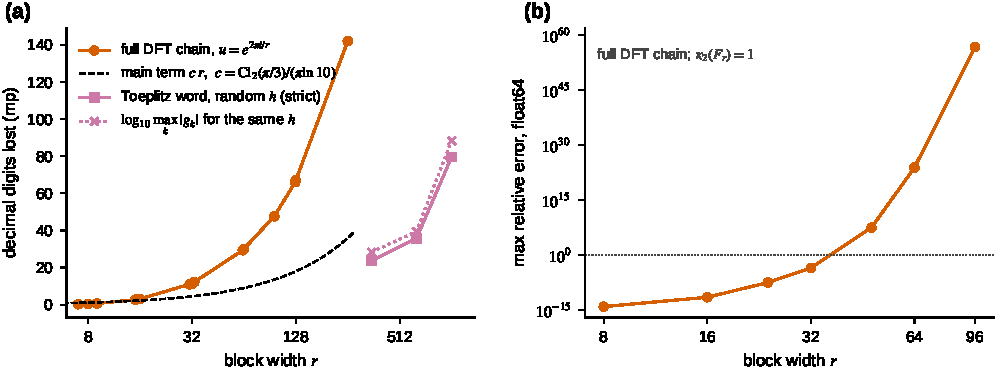
\includegraphics[width=\linewidth]{fig5_precision.pdf}
\caption{(a) Втрачені десяткові знаки в mp: повний ланцюжок DFT (таблиця~\ref{tab:mp}, усі ширини 7--256), Тепліцеве слово з випадковими $h$ (таблиця~\ref{tab:randtoep}) разом із $\log_{10}\max_k\abs{g_k}$ для тих самих $h$ і головний асимптотичний член $cr$, $c=\Cl(\pi/3)/(\pi\ln10)$. (b) Відносна похибка повного ланцюжка у float64 (таблиця~\ref{tab:float}); $\kappa_2(F_r)=1$. Підписи на рисунках англійською.}\label{fig:precision}
\end{figure}

\begin{table}[tb]
\centering\small
\caption{Втрата знаків по етапах (одна випадкова $x$). Локальна: етап на робочій точності, застосований до точного входу; ріст: $\log_{10}$ відношення максимального модуля проміжної координати до максимального модуля входу етапу.}\label{tab:stage}
\begin{tabular}{@{}rccccc@{}}
\toprule
$r$ & Етап & Локальна втрата & Накопичена втрата & Ріст & $\log_{10}$ норми виходу \\
\midrule
\gentable{2b}
\bottomrule
\end{tabular}
\end{table}

\paragraph{Втрата по етапах (\cref{tab:stage,fig:stagewise}).}
(1)~Діагональні етапи майже не втрачають знаків ($\le2$); уся втрата припадає на два Тепліцеві слова. (2)~Для $T^{\T}$ локальна втрата майже дорівнює росту проміжних значень (5{,}6 і 6{,}5; 17{,}5 і 19{,}1; 42{,}4 і 43{,}9): похибка поводиться як $\varepsilon$, помножене на найбільшу проміжну величину. (3)~Для $T$ локальна втрата перевищує ріст; вона порівнянна з $\log_{10}\kappa_2(T)$ плюс ріст (при $r=64$: $9{,}0+9{,}2\approx18$ проти 21{,}9), тобто тут додається підсилення похибки входу самим оператором. (4)~Повна втрата (таблиця~\ref{tab:mp}) становить 2{,}5, 3{,}3, 3{,}7 і 4{,}0 одиниці $\log_{10}\kappa_2(T)$ при $r=32,64,128,256$.

\begin{figure}[t]
\centering
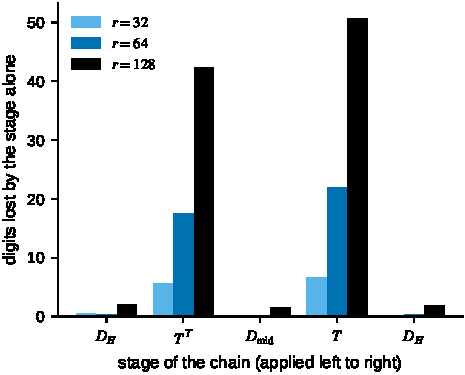
\includegraphics[width=0.55\linewidth]{fig6_stagewise.pdf}
\caption{Локальна втрата знаків по етапах ланцюжка $\Dh$, $T^{\T}$, $\Dmid$, $T$, $\Dh$ при $r=32,64,128$ (таблиця~\ref{tab:stage}).}\label{fig:stagewise}
\end{figure}

\paragraph{Де виникає ріст (таблиця~\ref{tab:growth} у додатку~\ref{app:tables}).}
Розклад росту з підрозділу~\ref{sec:stagewise} описує ріст, який може підсилювати округлення в $T^{\T}$ (де локальна втрата майже дорівнює росту); для $T$ втрата перевищує ріст, тож там розклад описує лише ріст. Його суми збігаються зі стовпцем росту таблиці~\ref{tab:stage} ($T^{\T}$: 6{,}5, 19{,}1, 43{,}9; $T$: 3{,}0, 9{,}2, 21{,}7). (1)~Увесь приріст рекордного максимуму $T^{\T}$ припадає на фазу міжблокових чанків, тобто на реплей displacement-DAG, побудованих з оберненого ряду $g$, а не на листові чи прямі шари. Для $T$ фаза чанків дає 67--84\%, решту~--- пряме трикутне слово базових блоків ширини 8 (нижче $v=10$ допустимого чанка немає, підрозділ~\ref{sec:counting}). (2)~Ріст розподілений по кількох рівнях рекурсії, а не зосереджений на одному. У $T^{\T}$ найбільший внесок дає зовнішній рівень $v=r$ (49--66\%); у $T$ внесок зміщується до середніх рівнів. Нульовий приріст на якомусь рівні (наприклад, $v=16$ для $T^{\T}$ при $r=128$) означає лише, що там не виникає нового рекорду, а не що рівень не впливає на похибку. (3)~Отже, великі проміжні величини локалізовано в displacement-реплеї чанків (ріст оберненого ряду $g$, підрозділ~\ref{sec:res-random}), і вони накопичуються по рівнях рекурсії.

\paragraph{Контроль точності фаз (таблиця~\ref{tab:phase} у додатку~\ref{app:tables}).}
Підвищення точності лише фази чанків зменшує втрату $T^{\T}$ приблизно на 14{,}5 і 37{,}5 знака при $r=64$ і $128$; підвищення точності лише прямої фази майже не впливає. Для $T$ зменшення становить приблизно 10{,}3 і 27{,}9 знака, але залишається втрата 11{,}6 і 22{,}6 знака. Отже, для перевірених входів і ширин точність чанків сильно впливає на похибку обох етапів, особливо $T^{\T}$. Це не адитивний розклад похибки: округлення у фазах і подальше підсилення взаємодіють, і залишок не можна назвати лише перенесенням без окремого контролю. Експеримент охоплює один випадковий вектор (seed $=r$) на ширину, фіксовані коефіцієнти DFT і $r=64,128$; інших розподілів коефіцієнтів і ширших випадків він не охоплює.

\subsection{Тепліцеве слово з випадковими коефіцієнтами}\label{sec:res-random}
Це тест загального Тепліцевого оператора $Tx$, а не DFT, виконаний у строгому режимі з трьома векторами і двома точностями (таблиця~\ref{tab:randtoep}). Для порівняння, варіант із пропуском нулів з одним вектором втрачав 23{,}6, 35{,}0 і 78{,}6 знака при $r=352,640,1024$.

\begin{table}[tb]
\centering\small
\caption{Тепліцеве слово, випадкові $h$, строгий режим.}\label{tab:randtoep}
\begin{tabular}{@{}rcccc@{}}
\toprule
$r$ & Точність, знаків & Макс. відносна похибка & Втрачено знаків & $\log_{10}\max_k\abs{g_k}$ \\
\midrule
\gentable{3}
\bottomrule
\end{tabular}
\end{table}

\paragraph{Механізм росту коефіцієнтів.}
Ряд $g$~--- обернений ряд до $h$ (\code{loc:reciprocal}), з якого будуються чанки; його радіус збіжності дорівнює найменшому модулю $\rho$ кореня $h(z)=\sum_k h_kz^k$. Отже, $\log_{10}\abs{g_k}$ росте з нахилом $\log_{10}(1/\rho)$.

\begin{table}[tb]
\centering\small
\caption{Корені $h(z)$ і ріст $g$ (\code{roots\_h.py}; корені~--- власні значення супровідної матриці, відносний залишок $\abs{h(z)}$ у найменших коренях $\le4\cdot10^{-14}$). Нахил підібрано на другій половині $k$.}\label{tab:roots}
\begin{tabular}{@{}rcccccc@{}}
\toprule
$r$ & \hd{$\rho=\min\abs{\text{корінь}}$} & \hd{Коренів усередині\\одиничного круга} & \hd{Нахил\\$\log_{10}\abs{g_k}$} & $\log_{10}(1/\rho)$ & \hd{$(r-1)\log_{10}(1/\rho)$} & \hd{Спостережений\\$\log_{10}\max_{k<r}\abs{g_k}$} \\
\midrule
\gentable{3a}
\bottomrule
\end{tabular}
\end{table}

Нахил збігається з $\log_{10}(1/\rho)$ до четвертого знака після коми, а прогноз $(r-1)\log_{10}(1/\rho)$ відрізняється від спостереженого максимуму менш ніж на один знак (таблиця~\ref{tab:roots}). Приблизно половина коренів лежить усередині одиничного круга; найменший модуль становить 0{,}82--0{,}86. Отже, для цих трьох вибірок ріст $g$ пояснюється найменшим коренем $h(z)$, а втрата знаків майже дорівнює $\log_{10}\max_k\abs{g_k}$. Розподілу $\rho$ для інших розподілів коефіцієнтів ми не досліджували.

\subsection{Фіксована топологія}\label{sec:res-topology}
Для кожного прогону ми обчислюємо SHA-256 від послідовності шарів, де кожен шар записано як його ASAP-раунд і список гейтів (тип M~--- масштабування або S~--- зсув, джерело, приймач). Аудит охоплює 12 ширин, 2 правила (адаптивне і чанк розміру 1) і 3 входи (seed $=r$, інший seed, $h=$ ones); повні дані наведено в таблиці~\ref{tab:topology} (додаток~\ref{app:tables}). Для кожної ширини і кожного правила хеш однаковий для всіх трьох входів. Отже, у строгому режимі типи гейтів, пари координат, порядок шарів, розклад за раундами, глибина і кількість гейтів є функціями лише ширини. Разом зі статичним аудитом підрозділу~\ref{sec:strict} це підтверджує для нашої реалізації вимогу препринту про фіксовану топологію. Для порівняння, у варіанті з пропуском нулів глибина при $r=64$ становила 24442 і 24452 для двох seed і 13969 для $h=$ ones.

\subsection{Глибина}\label{sec:res-depth}
Строгу ASAP-глибину виміряно на сітці з 12 ширин: 64, 128, 256, 288, 320, 336, 352, 384, 512, 640, 768, 1024 (\code{strict\_tables.py}; дані в \code{paper/data/strict\_tables.csv}).

\begin{table}[tb]
\centering\small
\caption{Строга ASAP-глибина: адаптивне правило проти чанка розміру 1. Останній стовпець~--- відношення глибин для залежного від значень варіанта з пропуском нулів (архівні дані).}\label{tab:depth}
\begin{tabular}{@{}rcrrcc@{}}
\toprule
$r$ & $b$ & Адаптивне & Чанк 1 & \hd{Адаптивне /\\чанк 1} & \hd{Варіант з пропуском нулів,\\адаптивне / чанк 1} \\
\midrule
\gentable{5}
\bottomrule
\end{tabular}
\end{table}

У строгому режимі адаптивне правило має глибину, не більшу, ніж чанк розміру 1, на всіх 12 ширинах сітки, і строго меншу, починаючи з $r=128$ (\cref{tab:depth,fig:depth}). Перетин між 320 і 336, помітний у варіанті з пропуском нулів, зникає: там чанк розміру 1 отримував перевагу, бо в DAG для чанків розміру 1 багато точкових множників дорівнюють нулю точно ($g(1)=6$ замість 8, $L(1)=18$ замість 28). Стрибок відношення між 320 і 336 збігається зі стрибком $b$ від 2 до 3 і зберігається в обох режимах. Ці висновки стосуються саме цієї сітки; для проміжних $r$ ми їх не стверджуємо. Глибина не монотонна за $r$: при $r=352$ вона менша, ніж при $r=320$, бо більший блок допускає більший чанк.

\begin{figure}[t]
\centering
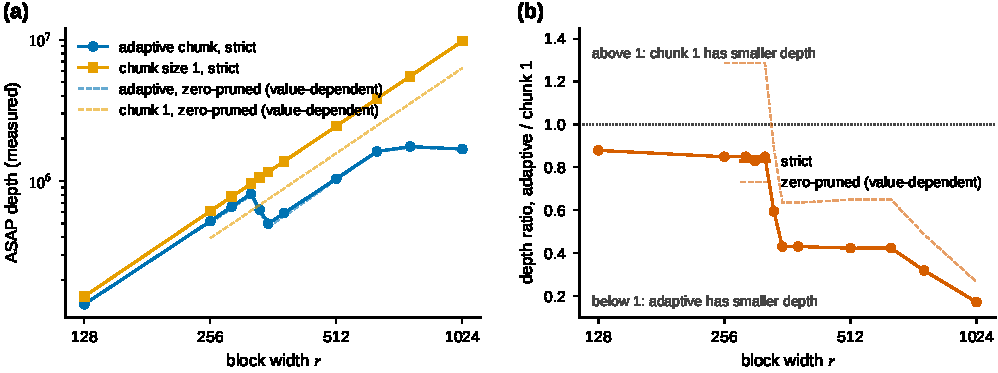
\includegraphics[width=\linewidth]{fig1_depth.pdf}
\caption{(a) Виміряна ASAP-глибина строгого слова для адаптивного правила і чанка розміру 1 (суцільні лінії) і та сама величина для залежного від значень варіанта з пропуском нулів (тонкі штрихові лінії, архівні дані). Логарифмічні осі. (b) Відношення глибин адаптивне / чанк 1; пунктир~--- рівність. Нижче 1 адаптивне правило має меншу глибину. У строгому режимі відношення менше 1 на всіх ширинах, починаючи з 128; перетин варіанта з пропуском нулів біля $r\approx330$~--- артефакт пропуску нулів. Дані: таблиця~\ref{tab:depth}.}\label{fig:depth}
\end{figure}

\paragraph{Модель глибини.}
Ми використовуємо рекурентність
\begin{equation}\label{eq:depth-model}
d(v)=d(\lfloor v/2\rfloor)+k^2L(b),\qquad k=\bigl\lceil\lfloor v/2\rfloor/b\bigr\rceil,
\end{equation}
з прямою вартістю $v(v+1)/2$ для блоків без допустимого чанка; $b$ визначається строгою таблицею $g(b)$, а $L(b)$~--- кількість шарів реплею однієї пари $b\times b$ у строгому режимі (\code{depth\_exact\_rule.py --strict}). Модель використовує виміряні $g(b)$ і $L(b)$ і йде лише гілкою $\lfloor v/2\rfloor$; для степенів двійки обидві гілки збігаються.

\begin{table}[tb]
\centering\small
\begin{minipage}[t]{0.48\linewidth}\centering
\caption{Модель строгої глибини проти виміряної ASAP-глибини (адаптивне правило).}\label{tab:model}
\begin{tabular}{@{}rrrc@{}}
\toprule
$r$ & Модель & ASAP & ASAP / модель \\
\midrule
\gentable{6a}
\bottomrule
\end{tabular}
\end{minipage}\hfill
\begin{minipage}[t]{0.48\linewidth}\centering
\vspace{0pt}
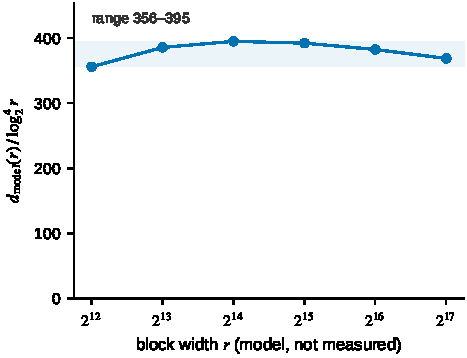
\includegraphics[width=\linewidth]{fig3_log4_law.pdf}
\captionof{figure}{Відношення $d_{\mathrm{model}}(r)/\log_2^4 r$ моделі строгої глибини на степенях двійки $2^{12}$--$2^{17}$; смуга позначає діапазон значень. Значення моделі, а не вимірювання. Дані: таблиця~\ref{tab:model-pow2}.}\label{fig:log4}
\end{minipage}
\end{table}

Модель точно збігається з вимірюванням на 10 з 12 ширин (таблиця~\ref{tab:model}). При $r=336$ і $352$ рекурсія доходить до непарних блоків $v\ge10$ (21 і 11), і модель, що йде лише гілкою $\lfloor v/2\rfloor$, занижує глибину. Це прямо підтверджує, що повна рекурентність має брати максимум по обох гілках, як у доведенні препринту~\eqref{eq:depth-rec}.

На степенях двійки $2^{12}$--$2^{17}$ модель дає $d_{\mathrm{model}}/\log_2^4 r$ у межах 356--395 (таблиця~\ref{tab:model-pow2} у додатку~\ref{app:tables}, рисунок~\ref{fig:log4}). Ці значення отримано з моделі; ASAP-слів таких ширин ми не будували. Оскільки модель побудовано на емпіричних $g(b)$ і $L(b)$, її збіг з вимірюваннями є перевіркою узгодженості, а не незалежним доведенням $O(\log^4 r)$. Евристика порядку величини
\begin{equation}\label{eq:heuristic}
g(b)\approx C\,b\log b\ \Rightarrow\ b=\Theta(v/\log v),\quad k=\Theta(\log v),\quad L(b)=\Theta(\log v),
\end{equation}
за якою один рівень дає внесок $\Theta(\log^3 v)$, а рівнів $\log_2 r$, пояснює, чому модель поводиться як $\log^4 r$, і відповідає доведенню верхньої межі в препринті. Шість майже сталих точок узгоджуються з $O(\log^4 r)$, але не встановлюють асимптотичної рівності.

\subsection{Вартість в однакових одиницях}\label{sec:res-cost}
У таблиці~\ref{tab:flops} наведено дійсні флопи (строгий режим, адаптивне правило, одиниці з підрозділу~\ref{sec:cost-units}).

\begin{table}[tb]
\centering\footnotesize
\setlength{\tabcolsep}{2.5pt}
\caption{Дійсні флопи. Відношення: DFT через слово до радікс-2 FFT, а також одне Тепліцеве слово до циркулянтного FFT і до прямого Тепліцевого множення.}\label{tab:flops}
\begin{tabular}{@{}rrrrrrrrr@{}}
\toprule
$r$ & \hd{Одне\\Тепліцеве\\слово} & \hd{DFT\\через\\слово} & \hd{Радікс-2\\FFT} & \hd{Тепліцеве\\через цирку-\\лянтний FFT} & \hd{Пряме\\Тепліцеве} & \hd{DFT через\\слово /\\FFT} & \hd{Слово /\\цирку-\\лянтний FFT} & \hd{Слово /\\пряме} \\
\midrule
\gentable{7}
\bottomrule
\end{tabular}
\end{table}

Кількість гейтів одного слова, поділена на $r^2$, становить 15{,}8, 56{,}7, 77{,}1, 74{,}9 і 61{,}6 при $r=64,\dots,1024$. Ця величина не стала, тож дані не встановлюють квадратичного закону вартості. На перевірених ширинах слово дорожче навіть за пряме множення (рисунок~\ref{fig:cost}). Це вартість окремого виконання слова; препринт так слово не використовує і переваги на цих ширинах не заявляє (підрозділ~\ref{sec:cost-units}). Препринт посилається на Alman і Rao~\citep{alman2023} з головним членом $(15/4)\,n\log_2 n$ дійсних операцій для DFT на степенях двійки; порівняно з цим еталоном розрив був би ще більшим.

\begin{figure}[t]
\centering
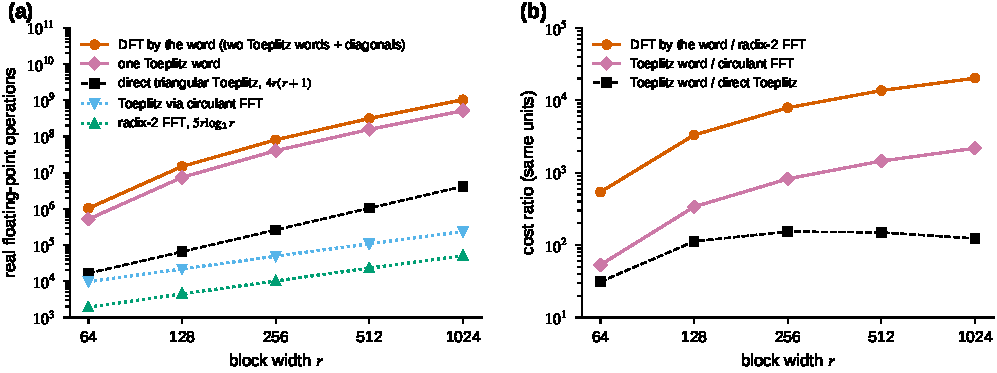
\includegraphics[width=\linewidth]{fig2_cost.pdf}
\caption{(a) Дійсні флопи DFT через слово, одного Тепліцевого слова, прямого Тепліцевого множення, Тепліцевого множення через циркулянтний FFT і радікс-2 FFT. (b) Відношення вартостей у тих самих одиницях. Дані: таблиця~\ref{tab:flops}.}\label{fig:cost}
\end{figure}

\paragraph{Компроміс між гейтами і глибиною при $r=512$ (рисунок~\ref{fig:tradeoff}).}
Строгий режим, три правила:
\begin{itemize}
\item адаптивне ($b=4$): глибина 1\,035\,044, 19\,638\,528 гейтів;
\item чанк розміру 1: глибина 2\,446\,116, 4\,647\,168 гейтів;
\item cap2 ($b\le2$): глибина 2\,059\,044, 22\,882\,560 гейтів.
\end{itemize}
Адаптивне правило і чанк розміру 1 утворюють компроміс: у чанка розміру 1 у 4{,}2 раза менше гейтів і в 2{,}4 раза більша глибина. cap2 гірше за адаптивне правило за обома показниками, тобто серед цих трьох правил воно доміноване. Перевірено лише три правила. Інші розміри чанків, різні правила на різних рівнях рекурсії або інший розклад можуть дати кращі точки, тож ми не стверджуємо, що жодне правило не мінімізує обидві величини.

\begin{figure}[t]
\centering
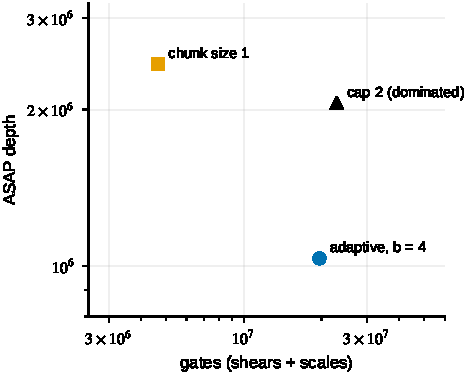
\includegraphics[width=0.5\linewidth]{fig4_tradeoff_r512.pdf}
\caption{Гейти і глибина при $r=512$ для трьох правил у строгому режимі. Обидві осі логарифмічні. Розкиду по входах немає, бо топологія фіксована.}\label{fig:tradeoff}
\end{figure}

\subsection{Раунди і конфлікти}\label{sec:res-rounds}
У строгому режимі (\code{rounds\_check.py}) виконання за раундами дає той самий результат, що й послідовне: різниця 0{,}0 при $r=16,32,48,64$. У межах раунду немає конфліктів координат: 0 при $r=256$ (779\,392 шари, 518\,948 раундів, 1{,}50 шару на раунд) і при $r=512$ (2\,074\,880 шарів, 1\,035\,044 раунди, 2{,}00 шару на раунд).

\subsection{Час і пам'ять нашої реалізації}\label{sec:res-time}
Один процес на ширину, float64, строгий режим, адаптивне правило, машина з підрозділу~\ref{sec:env}, команда \code{timing.py r}. Ми вимірюємо одне Тепліцеве слово на випадкових комплексних $h$ і $x$ (\code{numpy.default\_rng(r)}, дійсні та уявні частини \code{standard\_normal}, $h_0$ замінено на $\abs{h_0}+1$), а не повний ланцюжок DFT із двома словами і діагональними множниками. У коді RSS підписано як GB, але \code{ru\_maxrss}$/1024^2$ на Linux дає ГіБ; у таблицях ужито ГіБ.

Вимірювання з таблиці~\ref{tab:timing} зроблено 2026-10-14 у прогоні \code{full-20261013-r3}. Прогін виконує кроки послідовно, тож кроки \code{timing-64}, \dots, \code{timing-512} не перетиналися з іншими кроками прогону; кожен із них~--- окремий процес у чистому віртуальному середовищі (Python 3.12.3, numpy 1.26.4) з \code{OPENBLAS\_NUM\_THREADS} $=$ \code{OMP\_NUM\_THREADS} $=$ \code{MKL\_NUM\_THREADS} $=1$. Інших процесів на машині не контролювали. Чотири кроки разом тривали 24~с. Попереднє вимірювання тією самою командою, зроблене тоді, коли на машині працювали ще сім однопотокових обчислень (із 32 потоків), збережено без змін як запис тих умов у таблиці~\ref{tab:timing-hist} (додаток~\ref{app:tables}).

\begin{table}[tb]
\centering\small
\caption{Python-реалізація (\code{timing.py}), вимірювання 2026-10-14 без паралельних кроків прогону. Побудова: підготовка скалярів і розкладу.}\label{tab:timing}
\begin{tabular}{@{}rrccccc@{}}
\toprule
$r$ & Гейтів & \hd{Побудова\\слова, с} & \hd{Застосування\\до одного\\вектора, с} & \hd{Пікова\\пам'ять,\\ГіБ} & \hd{numpy.fft\\довжини $r$,\\мкс} & \hd{Щільне\\Тепліцеве\\множення\\(numpy), мкс} \\
\midrule
\gentable{8a}
\bottomrule
\end{tabular}
\end{table}

У цих прогонах вимірювання часу проміжні значення у float64 переповнюються при $r\ge256$, тож виходи не використовуються як перевірка правильності; час вимірює виконання того самого фіксованого списку гейтів у Python, а точну правильність і числову поведінку перевірено окремими експериментами вище. Кількість гейтів однакова в обох вимірюваннях і дорівнює сумі зсувів і масштабувань адаптивного слова в таблиці~\ref{tab:topology}. Відношення повторного часу до попереднього становить 0{,}81--0{,}88 для побудови, 0{,}81--1{,}00 для застосування і 0{,}73--0{,}81 для \code{numpy.fft}. Побудова слова в mp дорожча: 7--83~с при $r=127$--256 з 250--450 знаками в попередніх журналах (таблиця~\ref{tab:mp}) і 3--79~с у повторному прогоні. Ці числа описують нашу Python-реалізацію на цій машині, а не алгоритм препринту. Вони показують порядок величини: наша реалізація застосовує одне слово приблизно від $10^4$ ($r=64$) до $10^6$ ($r=512$) разів повільніше, ніж \code{numpy.fft} виконує все перетворення (і в повторному, і в попередньому вимірюванні), а пам'ять росте разом із кількістю гейтів. При $r=512$ слово будується за 13{,}2~с (15~с у попередньому вимірюванні).

% =====================================================================
\section{Обговорення}\label{sec:discussion}

\subsection{Показник і повна формула}\label{sec:disc-theta}
З $\delta$ із~\eqref{eq:delta} відношення головних множників дорівнює
\begin{equation}\label{eq:ratio}
\frac{n(\log n)^{\theta}(\log\log n)^{4-\theta}}{n\log n}=\frac{(\log\log n)^{3+\delta}}{(\log n)^{\delta}} .
\end{equation}
Воно прямує до нуля, тож заявлена межа справді є $o(n\log n)$. Проте при практичних $n$ воно велике. При $n=10^{300}$ з натуральними логарифмами ($\ln n\approx690{,}8$, $\ln\ln n\approx6{,}54$) відношення дорівнює $\approx279{,}446$ без урахування прихованих сталих (з $\log_2$ було б $\approx988$). Відношення стає меншим за 1 лише тоді, коли
\begin{equation}\label{eq:crossover}
\delta\,\ln\ln n>(3+\delta)\,\ln(\ln\ln n),\qquad\text{тобто при }\ln\ln n\approx4{,}81494\cdot10^{14}.
\end{equation}
Це не прогноз часу виконання, а пояснення, чому мала різниця показників не означає практичного прискорення. Числове значення $\theta$ перераховано в підрозділі~\ref{sec:constants}; наші скінченні локальні експерименти не перевіряють заявленої глобальної асимптотичної межі часу, для якої потрібне аналітичне або формальне доведення.

\subsection{Розрив між масштабами}\label{sec:disc-scale}
$m=10^6$ і $W_*=2^{71}$~--- параметри тензорної мережі, а не ширини локального компілятора. Локальні ширини в доведенні~--- перші $\ell$ непарних простих і один степінь двійки $2^e<2r_{\ell+1}$, $\ell=\Theta(\log n/\log\log n)$ (\code{all-lengths.tex:13--56}); ширини цих типів (непарні прості, як-от 7, 31 і 127, і степені двійки) частково покрито нашими тестами. Конкретна мережна рекурсія застосовується лише в секторах з $k\ge K=m(71+1)=72\,000\,000$ осями (\code{network.tex:494--498}), а $k\le\ell$ (\code{synchronization.tex:82}). Тоді $\ell\ge72\,000\,000$, і вже елементарна нижня межа $r_\ell\ge\ell+2$ показує, що найбільша локальна ширина перевищує 1024 більш ніж у 70 тисяч разів. Це зіставлення найбільшої ширини, а не твердження, що всі осі великі. Екстраполяція нашої числової поведінки на такі ширини не обґрунтована.

\subsection{Робота проти часу}
Препринт обмежує повний час, включно з підготовкою скалярів і роботою з індексами. Ми рахуємо гейти слова та їхні флопи, а час і пам'ять вимірюємо лише для нашої реалізації (\cref{tab:timing,tab:timing-hist}).

\subsection{Оптимізації, залежні від значень}\label{sec:disc-value}
Пропуск нульових множників не змінює оператора, тож для числової реалізації оператора він допустимий. Але він виходить за межі конструкції препринту, бо потребує тесту на нуль комплексного коефіцієнта, якого конструкція не використовує (\code{local.tex:42}), і змінює об'єкт вимірювання: глибина і робота стають властивостями пари (ширина, коефіцієнти), а не ширини. Методологічний урок прямий: залежний від значень варіант може породжувати структурні ефекти, яких немає в досліджуваній конструкції. У нашому випадку він породив хибний перетин глибин між $r=320$ і $336$ та хибний розкид глибини між seed (підрозділ~\ref{sec:strict}); усі наведені тут результати використовують строгу конструкцію. Вироджені входи ($h=$ ones) цікаві самі по собі, і їх слід аналізувати окремо, а не виключати; у строгому режимі вони дають ту саму структуру, що й загальні.

\subsection{Числова нестійкість}\label{sec:disc-instability}
Конструкцію препринту розраховано на точну арифметику, і стійкості препринт не заявляє. Наші дані показують, наскільки важливе це обмеження. У випадку Фур'є обумовленість Тепліцевого множника росте приблизно як $10^{cr}$, $c=\Cl(\pi/3)/(\pi\ln10)\approx0{,}1403$ (головний асимптотичний член скінченної обумовленості $\Dh$), а повний ланцюжок втрачає 3--4 такі одиниці, тобто близько $0{,}5\,r$ десяткових знаків (142 при $r=256$). У float64 ланцюжок непридатний уже з $r\approx32$. Звичайний FFT стійкий. Пряме виконання цього слова (з природним порядком вузлів) у скінченній точності потребувало б на перевірених ширинах кількості знаків, що росте приблизно лінійно з $r$; це змінює бітову вартість. Препринт нічого не стверджує про бітову складність (\code{introduction.tex:101}), тож це не суперечність, а кількісна ілюстрація обмеження, яке він сам називає. Висновок стосується лише локальної складової: він не означає, що повний алгоритм нестійкий у будь-якій реалізації, і не встановлює нижньої межі вартості інших модифікацій.

\subsection{Нижні межі}
Межі Morgenstern і Ailon стосуються обмежених коефіцієнтів, унітарних гейтів або обмеженої обумовленості. Наші дані показують, що локальний компілятор справді лежить поза цими рамками: обумовленість його множників росте експоненційно з $r$. Це узгоджується з тим, що межі на нього не поширюються, але нічого не говорить про правильність мережі.

\subsection{Що випливає для препринту}\label{sec:implications}
У межах перевіреного діапазону локальна складова поводиться так, як заявлено: реалізований оператор дорівнює $F_r(u)$ (доведено обчисленням у $\Q(\zeta_N)$ для восьми ширин 4--32; для інших перевірених $r$~--- узгоджується з рівністю), топологія строгого слова залежить лише від $r$, а модель глибини сумісна з $O(\log^4 r)$. Розбіжностей із твердженнями препринту ми не знайшли. Це не підтверджує і не спростовує головної теореми, ефект якої походить від мережі. Для перевірки самого доведення препринту потрібен аудит мережі й синхронізації; звірку Lean-означень завершено в обсязі підрозділу~\ref{sec:lean}. Наші вимірювання кількісно описують для локальної складової обмеження, які препринт називає сам (величезні сталі, точна арифметика; \code{introduction.tex:67}, \code{:101}), і узгоджуються з практичними зауваженнями Recht~\citep{recht2026}; про правильність препринту вони нічого не говорять.

% =====================================================================
\section{Обмеження і загрози валідності}\label{sec:limitations}

\paragraph{Обсяг перевірок.}
Повний DFT доведено обчисленням у $\Q(\zeta_N)$ на восьми ширинах від 4 до 32; у $\Fp$ (необхідна умова) його перевірено для всієї матриці на десяти вибраних ширинах від 9 до 128, для кількох векторів при $r=255,256,512$ і окремо в потоковому режимі при $r=1024$ (ті самі два вектори у двох полях); у mp~--- при $r\le256$. $C$-слоти доведено обчисленням у $\Q(\zeta_N)$ при $r=4,8,16$, перевірено в $\Fp$ для всієї матриці при $r=16,31,32,33,64$ і вибірково при $r=128$, а в mp~--- при $r\le256$. Тепліцеве слово з випадковими $h$ перевірено при $r\le1024$; глибину виміряно при $r\le1024$ і змодельовано до $r=2^{17}$. У mp при $r=96,127,256$ і в $\Fp$ при $r=255,256,512$ перевірено кілька випадкових векторів, а не всю матрицю; у $\Fp$ при $r=127$ перевірено всі базисні вектори.

\paragraph{Сила доказу.}
Точні перевірки в $\Fp$~--- необхідна умова, а не доведення комплексної рівності; доведеннями обчисленням є лише перевірки в $\Q(\zeta_N)$. Збіг у mp~--- лише числова узгодженість.

\paragraph{Глибина.}
ASAP-глибина~--- конкретний розклад, а не оптимум і не нижня межа. Еквівалентність нашого правила чанка правилу препринту встановлено лише для $b\le1024$ (підрозділ~\ref{sec:chunk}). Модель глибини використовує емпіричні $g(b)$ і $L(b)$ і йде лише гілкою $\lfloor v/2\rfloor$.

\paragraph{Аналіз нестійкості.}
Вимірювання по етапах описують спостережений розподіл втрати знаків (таблиця~\ref{tab:stage}); розклад росту описує прирости рекордного максимуму по рівнях рекурсії і фазах (таблиця~\ref{tab:growth}); а контроль точності фаз (таблиця~\ref{tab:phase}, $r=64,128$) вимірює чутливість похибки до точності міжблокових чанків для перевірених входів. Разом ці діагностики не дають повного причинного розкладу похибки округлення. Підготовки коефіцієнтів цей контроль не охоплює, і для $T$ після нього залишається значна втрата. Не зроблено: розкладу до рівня окремих чанків, контролю для інших розподілів коефіцієнтів із можливим взаємним скороченням і ширин понад $r=128$.

\paragraph{Вартість.}
Підготовку скалярів, індекси і пам'ять виміряно лише для нашої Python-реалізації; флопи пораховано за стандартною схемою без спеціальних коефіцієнтів.

\paragraph{Lean.}
Ми повторно перевірили замикання головної цілі, аксіоми і відповідність означень \code{DFTGoal}/\code{ConvGoal}/\code{RAM} формулюванням препринту. Формалізація доводить потрібну межу через іншу мережу; \code{network.tex}, $\Delta$ і \code{net:tensor-bound} нею не перевіряються. Тіл доведень ми не перечитували; відповідність \code{Bill} фізичній word-RAM залишається модельним судженням; окремої теореми симуляції немає. Це відтворення чужої механічної перевірки, а не наше власне незалежне доведення.

\paragraph{Головна теорема.}
Числове значення $\theta$ перераховано (підрозділ~\ref{sec:constants}), але головний асимптотичний виграш, мережу, синхронізацію, алгоритм для довжин усіх розмірів і синтез локальними експериментами не перевірено.

\paragraph{Загрози валідності.}
Точні перевірки виконує \code{generic\_word.py}, тоді як чисельні використовують \code{mp\_exact}/\code{mp\_compiler} і \code{conv\_dag}/\code{rounds}. Це окремі реалізації однієї описаної конструкції, тож рівність у точному полі безпосередньо стосується саме точного перевірника. Додаткове порівняння послідовностей шарів і пар координат (без коефіцієнтів) показало, що три строгі конструктори збігаються при $r=4,7,8,9,12,15,16,31,32,33,64,128$ для $h_k=1/(k+1)$; це підтримує структурну відповідність, але не доводить збігу їхніх коефіцієнтів і не є твердженням для всіх ширин. Власний розклад зсуву, рання зупинка правила чанка і ASAP-розклад~--- рішення реалізації; їхні перевірені межі наведено вище. Фазові діагностики і діагностики випадкового Тепліцевого слова використовують один seed на ширину; ширшого статистичного узагальнення не заявлено. Час залежить від машини і від одночасного навантаження.

% =====================================================================
\section{Доступність даних і коду}\label{sec:availability}
Код, дані і сирі журнали повного прогону \code{full-20261013-r3} разом із його маніфестом і хешами доступні за адресою \url{https://github.com/cyberdid/fft-power-saving-verification} за ліцензією Apache License 2.0. Шляхи нижче задано відносно кореня цього репозиторію.

\begin{itemize}
\item \code{release/README\_REPRODUCE.md}: кроки відтворення і відповідність скриптів таблицям.
\item \code{release/run\_all.sh quick|full}: ізольований прогін, тобто копія джерел, потім сирі результати, потім CSV-файли цього прогону, потім звірка з ними всіх таблиць рукопису, потім рисунки з тих самих CSV-файлів. Кожен прогін має власний каталог і маніфест команд, кодів завершення і хешів. Режим \code{full} виконує всі 135 кроків; режим \code{quick} явно пропускає шість найдовших експериментів і тому не підтверджує повного відтворення. Перерваний прогін можна продовжити в тому самому середовищі; при продовженні перевіряється, що зафіксовані джерела, середовище і результати завершених кроків не змінилися.
\item \code{release/evidence/full-20261013-r3/}: сирі журнали, агреговані дані, рисунки, freeze середовища і маніфест повного прогону, використаного в цій статті; маніфест містить SHA-256 кожного зафіксованого файлу джерел, кожного журналу і кожного виходу. Файли побайтово ідентичні файлам прогону і тому зберігають абсолютні шляхи машини, на якій його виконано. Криві порівняння для варіанта з пропуском нулів на рисунку~\ref{fig:depth} архівні і позначені відповідно.
\item \code{paper/data/supplemental/fp1024/}: дані, журнали та інструкції з відтворення окремого потокового $\Fp$-тесту при $r=1024$ (\code{paper/scripts/stream\_exact\_dft.py}), який не входить до 135 кроків.
\item \code{release/requirements-lock.txt}: зафіксовані прямі й транзитивні залежності, встановлені в чисте середовище з успішним \code{pip check}; \code{release/requirements-full-freeze.txt}: повний freeze середовища розробки (запис, а не lock-файл); \code{release/ENVIRONMENT.txt}.
\item \code{release/lean/}: \code{lean-toolchain}, \code{lakefile.lean}, \code{lake-manifest.json}, \code{AxiomCheck.lean}, \code{MODEL\_AUDIT.md} і журнали збірки.
\item \code{release/SHA256SUMS}: контрольні суми коду, даних і рисунків цієї версії; вони засвідчують цілісність зафіксованих файлів, а не доведення будь-якої теореми.
\end{itemize}
Код міститься в \code{allength/} (серед іншого \code{conv\_dag.py} з прапорцем \code{KEEP\_ZERO\_MULTIPLIERS}, \code{mp\_exact.py} з \code{ROOT\_SIGN}, \code{exact\_field.py}, \code{generic\_word.py}, \code{rounds.py}, \code{mp\_compiler.py}, \code{compiler.py}, \code{depth\_recurrence.py}); скрипти~--- у \code{paper/scripts/}, агреговані дані~--- у \code{paper/data/*.csv}. Препринт доступний у репозиторії \url{https://github.com/openai/math} (коміт каталогу 301488868, HEAD fd4aeeb).

% =====================================================================
\section{Висновок}\label{sec:conclusion}
Ми незалежно перевірили локальний компілятор препринту OpenAI у строгій формі, де топологія залежить лише від ширини, і підтвердили цю властивість аудитом коду і хешами структури. Для восьми ширин від 4 до 32 ми довели обчисленням у циклотомічних полях, що матриця точного конструктора дорівнює $F_r(u)$. Для вибраних ширин до $r=512$ і в окремому потоковому тесті при $r=1024$ точні перевірки в скінченних полях дають необхідну умову (вибірково при $r=255,256,512,1024$), а арифметика високої точності до $r=256$ узгоджується з рівністю. Шлях через $C$-слоти (наш розклад зсуву; розщеплення і спряження через DAG з оберненими коренями, як у препринті) доведено обчисленням при $r=4,8,16$.

У скінченній точності ця точна конструкція сильно нестійка; препринт стійкості не заявляє, тож це не суперечить жодному його твердженню. Обумовленість Тепліцевого множника у випадку Фур'є росте приблизно як $10^{cr}$, $c\approx0{,}1403$ (головний асимптотичний член скінченної обумовленості, через функцію Клаузена); повний ланцюжок втрачає близько $0{,}5\,r$ десяткових знаків, майже всі~--- у двох Тепліцевих словах, і у float64 непридатний уже з $r\approx32$, хоча $\kappa_2(F_r)=1$. Виміряна глибина строгого слова до $r=1024$ і модель глибини до $2^{17}$ сумісні з верхньою межею $O(\log^4 r)$. Вартість окремого виконання слова в дійсних флопах на перевірених ширинах на два--чотири порядки перевищує FFT і перевищує навіть пряме множення; препринт так слово не використовує (підрозділ~\ref{sec:cost-units}). Варіант, що відкидає точно нульові множники, залежить від значень і породжує ефекти глибини, відсутні в строгій конструкції; тому всі результати тут отримано для останньої.

Наші локальні експерименти не перевіряють головного асимптотичного виграшу з $\theta$. Перекомпільована нами Lean-формалізація OpenAI доводить \code{DFTGoal} з потрібною верхньою межею через іншу мережу; конкретна \code{network.tex} та її $\Delta$ нею не перевіряються. Звірку означень завершено в обсязі підрозділу~\ref{sec:lean}; адекватність \code{Bill} щодо фізичної RAM залишається модельним судженням, а тіл доведень ми построково не перечитували. Наші результати не спростовують теореми і не є незалежним доведенням її головного ефекту; вони окреслюють перевірену локальну реалізацію та межі її використання у скінченній точності.

% =====================================================================
{\raggedright
\bibliographystyle{plainnat}
\bibliography{../refs}
\par}

% =====================================================================
\appendix

\section{Додаткові таблиці}\label{app:tables}

\begin{table}[tb]
\centering\small
\caption{Розклад росту проміжних величин по рівнях і фазах (одна випадкова $x$, seed $=r$; ріст у $\log_{10}$). В останньому стовпці наведено прирости за шириною блоку $v$.}\label{tab:growth}
\begin{tabularx}{\linewidth}{@{}rcccc L@{}}
\toprule
$r$ & Етап & Ріст & \hd{У фазі\\чанків} & \hd{У прямому\\слові} & Розподіл по рівнях $v$ (приріст) \\
\midrule
\gentable{2c}
\bottomrule
\end{tabularx}
\end{table}

\begin{table}[tb]
\centering\small
\caption{Втрачено знаків при DPS, коли вибрана фаза виконується на еталонній точності, а решта~--- на DPS; у дужках~--- зміна відносно «усе на DPS».}\label{tab:phase}
\begin{tabular}{@{}rccccc@{}}
\toprule
$r$ & Етап & DPS & Усе на DPS & \hd{Еталонна\\фаза чанків} & \hd{Еталонна\\пряма фаза} \\
\midrule
\gentable{2d}
\bottomrule
\end{tabular}
\end{table}

\begin{table}[tb]
\centering\small
\begin{minipage}[t]{0.40\linewidth}\centering
\caption{Модель строгої глибини на степенях двійки (значення моделі, а не вимірювання).}\label{tab:model-pow2}
\begin{tabular}{@{}rrrc@{}}
\toprule
$r$ & $b$ & $d_{\mathrm{model}}(r)$ & $d_{\mathrm{model}}/\log_2^4 r$ \\
\midrule
\gentable{6b}
\bottomrule
\end{tabular}
\end{minipage}\hfill
\begin{minipage}[t]{0.57\linewidth}\centering
\caption{Попереднє вимірювання часу (\code{timing.py}), зроблене тоді, коли на машині працювали ще сім однопотокових обчислень. Стовпці~--- як у таблиці~\ref{tab:timing}.}\label{tab:timing-hist}
\setlength{\tabcolsep}{2.5pt}
\begin{tabular}{@{}rrccccc@{}}
\toprule
$r$ & Гейтів & \hd{Побуд.,\\с} & \hd{Застос.,\\с} & \hd{Пам.,\\ГіБ} & \hd{fft,\\мкс} & \hd{Щільне,\\мкс} \\
\midrule
\gentable{8}
\bottomrule
\end{tabular}
\end{minipage}
\end{table}

\begin{table}[tb]
\centering\small
\caption{Аудит топології строгого слова: 12 ширин $\times$ 2 правила $\times$ 3 входи (seed $=r$, інший seed, $h=$ ones). Останній стовпець показує, чи однаковий хеш структури для трьох входів.}\label{tab:topology}
\begin{tabular}{@{}rlrrrl@{}}
\toprule
$r$ & Правило & Глибина & Шарів & Гейтів & Однаковий хеш \\
\midrule
\gentable{4}
\bottomrule
\end{tabular}
\end{table}

\clearpage
\section{Доведення і виведення}\label{app:proofs}

\subsection{Ненульовість коефіцієнтів розщеплення}\label{app:kappa}
\begin{proof}[Доведення леми~\ref{lem:split}]
Оскільки $\kappa=1+\abs{\mu}^2$ дійсне і $\kappa\ge1$, маємо $t_1=\kappa\ne0$. За оберненою нерівністю трикутника $\abs{t_2}=\abs{\kappa-\mu}\ge\abs{\kappa}-\abs{\mu}=1+\abs{\mu}^2-\abs{\mu}$. Виділяючи повний квадрат,
\[
1+\abs{\mu}^2-\abs{\mu}=\Bigl(\abs{\mu}-\tfrac12\Bigr)^2+\tfrac34\ \ge\ \tfrac34>0 .
\]
Отже, $t_2\ne0$, і $t_1+t_2=\mu$ для кожного $\mu$, включно з $\mu=0$. Міркування використовує те, що $\mu\bar\mu=\abs{\mu}^2$~--- невід'ємне дійсне число; тому воно не переноситься на $\Fp$, де ненульовість $t_1,t_2$ натомість перевіряється при кожному оберненні (підрозділ~\ref{sec:exact}).
\end{proof}

\subsection{Асимптотика Клаузена для \texorpdfstring{$\log_{10}\kappa_2(D_H)$}{log10 kappa2(DH)}}\label{app:clausen}
Нагадаємо, що $\Cl(\varphi)=-\int_0^{\varphi}\log\abs{2\sin(t/2)}\,dt$; її максимум на $[0,2\pi]$ досягається при $\varphi=\pi/3$, $\Cl(\pi/3)\approx1{,}01494$, і $\Cl(2\pi-\varphi)=-\Cl(\varphi)$.
\begin{proposition}\label{prop:clausen}
Для $u=e^{2\pi i/r}$ і $\Dh=\diag(H_0,\dots,H_{r-1})$
\[
\log_{10}\kappa_2(\Dh)=\frac{r}{\pi}\,\frac{\Cl(\pi/3)}{\ln10}+o(r)\qquad(r\to\infty).
\]
\end{proposition}
\begin{proof}
Для діагональної матриці $\kappa_2(\Dh)=\max_k\abs{H_k}/\min_k\abs{H_k}$. Оскільки $\abs{1-e^{2\pi is/r}}=2\sin(\pi s/r)$ при $0<s<r$,
\[
\ln\abs{H_k}=\sum_{s=1}^{k}\ln\bigl(2\sin(\pi s/r)\bigr).
\]
Доданок від'ємний при $\pi s/r<\pi/6$ і при $\pi s/r>5\pi/6$ і додатний між ними; отже, $\ln\abs{H_k}$ мінімальне при $k\approx r/6$ і максимальне при $k\approx5r/6$. Наближаючи суму інтегралом (підінтегральна функція має на кінцях лише інтегровні логарифмічні особливості, тож похибка суми Рімана є $o(r)$) і підставляючи $t=x/2$, маємо
\[
\ln\abs{H_k}=\frac{r}{\pi}\int_0^{\pi k/r}\ln(2\sin t)\,dt+o(r)=-\frac{r}{2\pi}\,\Cl\Bigl(\frac{2\pi k}{r}\Bigr)+o(r)
\]
рівномірно за $k$. При $2\pi k/r=5\pi/3$ значення дорівнює $-\frac{r}{2\pi}\Cl(5\pi/3)=\frac{r}{2\pi}\Cl(\pi/3)$, а при $2\pi k/r=\pi/3$~--- $-\frac{r}{2\pi}\Cl(\pi/3)$. Різниця дорівнює $\frac{r}{\pi}\Cl(\pi/3)+o(r)$; ділення на $\ln10$ дає твердження з $c=\Cl(\pi/3)/(\pi\ln10)=0{,}14030576$.
\end{proof}
Скінченні значення в таблиці~\ref{tab:cond}~--- точні різниці часткових сум; вони відрізняються від $cr$ на $o(r)$, наприклад на $10^{-4}$ при $r=1024$.

\subsection{Локалізація для \texorpdfstring{$\mathbb{F}_p$}{Fp}}\label{app:localisation}
\begin{proof}[Доведення твердження~\ref{prop:localisation}]
Нехай $p=kN+1$~--- просте і $\omega\in\Fp$ має мультиплікативний порядок $N$. Оскільки $p\nmid N$, $\omega$~--- корінь $\Phi_N$ за модулем $p$, і $\zeta_N\mapsto\omega$ задає сюр'єктивний гомоморфізм кілець $\phi:\Z[\zeta_N]\cong\Z[x]/(\Phi_N)\to\Fp$ з ядром $\mathfrak p$, яке є простим ідеалом. Нехай $R=\Z[\zeta_N]_{\mathfrak p}\subset\Q(\zeta_N)$~--- локалізація, тобто дроби $a/b$ з $a,b\in\Z[\zeta_N]$ і $b\notin\mathfrak p$. Тоді $\phi$ однозначно продовжується до гомоморфізму кілець $\phi:R\to\Fp$, $\phi(a/b)=\phi(a)\phi(b)^{-1}$; раціональні сталі зі знаменниками, взаємно простими з $p$, лежать у $R$.

Індукцією вздовж нерозгалуженої програми покажемо, що кожне проміжне значення $z$ лежить у $R$ і що значення, обчислене в $\Fp$, дорівнює $\phi(z)$. Входи і сталі цю умову задовольняють. Кільцеві операції зберігають $R$ і комутують з $\phi$. Якщо $z\in R$ обертається і обчислення в $\Fp$ обертає $\phi(z)\ne0$, то $z\notin\mathfrak pR$, отже, $z$~--- оборотний елемент локального кільця $R$, $z^{-1}\in R$ і $\phi(z^{-1})=\phi(z)^{-1}$. Таким чином, вихід у $\Fp$ є образом виходу в $\Q(\zeta_N)$. Якщо останній дорівнює $F_r(\zeta_r)$, то перший дорівнює $F_r(\phi(\zeta_r))$; від супротивного, розбіжність у $\Fp$ означає розбіжність над $\Q(\zeta_N)$, тоді як збіг у $\Fp$ не виключає ненульової різниці, що лежить у $\mathfrak pR$.

Комплексне спряження на $\Q(\zeta_N)$~--- це автоморфізм $\sigma:\zeta_N\mapsto\zeta_N^{-1}$. DAG, обчислений з оберненими коренями, обчислює $\sigma(\mu)=\bar\mu$ над $\Q(\zeta_N)$, а той самий DAG, обчислений у $\Fp$ з $\omega^{-1}$ замість $\omega$, за наведеним міркуванням обчислює $\phi(\sigma(\mu))$. Отже, перевірка шляху через $C$-слоти в $\Fp$ перевіряє образ того самого спряженого виразу, хоча саме поле $\Fp$ не має нетривіального автоморфізму.
\end{proof}

\section{Підсумок аудиту формулювання в Lean}\label{app:lean}
У таблиці~\ref{tab:lean} підсумовано звірку означень Lean з препринтом (підрозділ~\ref{sec:lean}). Тіл доведень не перечитували; їхню коректність для цих означень перевіряє ядро Lean.

\begin{table}[tb]
\centering\small
\caption{Означення Lean проти препринту. $G$ = \code{Goal.lean}, $R$ = \code{RAM.lean}, $C$ = \code{FourierCircuit/Core.lean}.}\label{tab:lean}
\begin{tabularx}{\linewidth}{@{}P{0.27\linewidth}LP{0.25\linewidth}@{}}
\toprule
Означення Lean (файл) & Зміст & Висновок \\
\midrule
\code{zeta}, \code{fourierMatrix} ($C$); \code{dft} ($G$) & $\zeta_n=\exp(2\pi i/n)$; $(\zeta_n^{jk})$; ненормоване $F_nx$ & Відповідає \code{introduction.tex} \\
Сталі $m$, $W_*$, $\Delta$, $\lambda$, $\theta$ ($G$) & Ті самі точні сталі, що й у~\eqref{eq:constants} & Відповідає \\
\code{paperTime}, \code{decimalTime} ($G$) & $n(\ln n)^{\theta}(\ln\ln n)^{4-\theta}$; показник $1-10^{-13}$; натуральні логарифми & Відповідає \code{thm:main}, \code{cor:decimal} \\
\code{DFTProgram} ($G$) & Для всіх $n>0$: порядок кореня $0<D<1024\,n^3$ обчислюється й оплачується в моделі; $\code{d.work}+1+\code{result.work}\le W(n)$; результат $=\code{dft}\,n\,x$ для всіх $x$ & Відповідає; порядок кореня обчислюється в моделі (сильніше) \\
\code{TimeBounds}, \code{DFTGoal} ($G$) & $W=O(\code{paperTime})$, $W=O(\code{decimalTime})$, $W=o(n\log n)$; фіксовані \code{order}, \code{solve}, $W$ & Відповідає \\
\code{ConvGoal} ($G$) & Білінійні добутки дозволено (\code{Prog true}); результат~--- лінійна згортка & Відповідає; сильніше (межа кореня, лише білінійні добутки) \\
\code{Paint}, \code{Bill}, атоми ($R$) & Окремі регістри скалярів і даних; кожен атом коштує 1; \code{inv} лише на скалярах з умовою ненульовості; немає комплексних сталих і атомів $\C\leftrightarrow\mathbb N$; розгалуження лише за цілими & Відповідає; теореми симуляції для word-RAM немає \\
\code{receipt} & $D=\code{receipt}(n)<8\,n^3$ у варіантах \code{\_order} & Формула відрізняється від $D_*$ (\code{eq:master-root}); межу виконано \\
Внутрішня мережа (\code{lunch\_big}, \code{alpha\_theta}) & 32 двійкові координати на множник, 4060 трійок, межа $2^{50}$; $W=O\bigl(n(\ln n)^{\alpha}(\ln\ln n)^2\bigr)$, $\alpha=1-2\cdot10^{-11}<\theta$ & Відрізняється від \code{network.tex}; $\Delta$ і \code{net:tensor-bound} не перевірено \\
Аксіоми (усі чотири головні теореми) & \code{propext}, \code{Classical.choice}, \code{Quot.sound} & Без \code{sorry}; 89 модулів у замиканні імпортів \\
\bottomrule
\end{tabularx}
\end{table}

\end{document}
